%%%%%%%%%%%%%%%%%%%%%%%%%%%%%%%%%%%%%%%%%%%%%%%%%%%%%%%%%%%%%%%%%%%%%%%

\newlength{\barchartwidth}
\setlength{\barchartwidth}{6.5cm}

%%%%%%%%%%%%%%%%%%%%%%%%%%%%%%%%%%%%%%%%%%%%%%%%%%%%%%%%%%%%%%%%%%%%%%%
\section{Experimental study}\label{sec:Experiment}

%%%%%%%%%%%%%%%%%%%%%%%%%%%%%%%%%%%%%%%%%%%%%%%%%%%%%%%%%%%%%%%%%%%%%%%
\subsection{Overview of experiments}\label{sec:Experiment.Overview}

We conducted three experiments, one for each of the initial problems outlined in Section~\ref{sec:schema}: P1 (action interpolation), P2 (action transfer) and P3
(shape transfer). Each experiment test all combinations of information (G,A,E) and learning algorithm (LWPR, KDE, KDEF) (see Table~\ref{tab:algs}). The structure of these experiments reflects the structure of our hypotheses: H1-H3.

{\bf Experiment P1 (action interpolation):} tests hypothesis. {\em {\bf H1}: a modular learning approach can outperform physics engines for prediction of rigid body motion for a variety of objects.} In the experiment each learning method was used to learn a specialised predictor for each object and the results were compared to the predictions of a physics simulator that had also been tuned to each object. In these experiments we also compared, where relevant, the effects of different parameterisations of rigid body transformations.

{\bf Experiment P2 (action transfer):} tests the hypothesis {\em {\bf H2}: learned predictions can be transferred to novel actions.} The learners were trained with a reduced action set on a non-symmetric object and then tested on that object with actions which fall well outside the convex hull of the training set. We performed this in simulation and with a real object.

{\bf Experiment P3 (shape transfer):} tests hypothesis. {\em {\bf H3}: learned predictions can be transferred to object shape.} Learners were trained on one or more objects, and tested on an object of different shape. Transfer was tested both in simulation and with real objects.

%We have explored the ways in which various combinations of input information
%and learning techniques can make predictions, through three sets of experiments.
%The experiments use a combination of real training and test data collected
%from our robot setup (described in Section~\ref{sec:Experiment.Setup}) and
%synthetic data from a simulation environment
%which has the benefit of perfectly known ground-truth.

%Experiments~L1, L2 and~L3 (see Section~\ref{sec:Results.Learning}) show how our various approaches can (L)earn to make accurate predictions about the motions of previously observed objects, including a polyflap, a box and a cylinder. Thus they test Hypothesis~1 and the interpolative aspect of Hypothesis~2. Experiment~A (see Section~\ref{sec:Results.Action}) compares the capabilities of the different approaches to predict
%the consequences of novel pushing (A)ctions which are completely different from those encountered during training. Experiment~A therefore tests the extrapolative part of Hypothesis~2. Experiments~S1 and~S2 (see Section~\ref{sec:Results.Shape}) compare the performance of the approaches in very challenging (S)hape generalization problems, where the the systems are tasked with making predictions about novel shapes which are very different to those encountered during training. Experiment~S3 tests the ability to interpolatively generalise when small variations in shape induce larger variations in behaviour. The experiments~S therefore test Hypothesis~3.

%Additionally, Experiments~L1-3 (Section~\ref{sec:Results.Learning}) investigate
%various parameters of the learning and prediction techniques.
%Each technique was trained on small, medium and large data sets
%to demonstrate that the methods converge.
%KDE techniques were attempted with a single global factor,
%a combination of two factors (global and agent),
%and multiple factors.
%We also compare results for different KDE kernel types and $SO(3)$
%parameterisations (see Section~\ref{sec:Implementation.kde}):
%Gaussian kernels with 1) quaternion and 2) Euler angle parameterisations,
%as well as 3) von Mises-Fisher kernels.
%We assess the performance of the LWPR regression method by using three versions --
%one that incorporates information equivalent to the KDE single ``global'' factor,
%and two others that include as inputs the additional information that is
%used to train the 2 factor and multiple factor KDEF predictors.

%To quantify the effect of factorising $p_{qs}$
%(equation~\eqref{eq:Learning.density}) as a product of densities
%we also include results from two sets of variants of the single factor case,
%denoted by KDE-GA and KDE-GAE.
%Both of these variants use a single factor,
%but with an augmented input space compared to the KDEF cases.
%For KDE-GA, information equivalent to that used by the agent factor was appended.
%For KDE-GAE, as well as agent information,
%the transformations used as input by the environment factors were also included,
%so that KDE-GAE estimated $p_{qs}$ directly in the form given by
%equation~\eqref{eq:Learning.density}.
%Again these two variants were tested with the quaternion, Euler angle, and von Mises-Fisher parameterisations.
%Note that KDEF with a single global factor (i.e.\ KDEF-G)
%and KDE-G are identical, hence KDE-G is not shown in the results.

%The results of Experiments~L (Section~\ref{sec:Results.Learning})
%show that the KDE methods perform best with Gaussian kernels
%and with a quaternion parametrisation of $SO(3)$.
%Hence, in Section~\ref{sec:Results.Action} and Section~\ref{sec:Results.Shape}
%only results for Gaussian and quaternion versions of KDE methods are presented.
%Likewise, we only show results of LWPR techniques
%using Euler angle $SO(3)$ parameterisations,
%since these result in a lower dimensional input space
%under which LWPR performs better.


%%%%%%%%%%%%%%%%%%%%%%%%%%%%%%%%%%%%%%%%%%%%%%%%%%%%%%%%%%%%%%%%%%%%%%%
\subsection{Experimental setup}\label{sec:Experiment.Setup}

In each learning trial a robot finger moved in a straight line to push
an object for 10 seconds, making contact at a randomly selected point
on its surface (Figure~\ref{fig:Setup}). Video and finger position were captured at 30Hz, including a 1 second buffer at either end of the finger trajectory. Learning used the pose of the object in every other frame estimated using a particle filter tracker \cite{morwald_edge_2009}. For test trials the trajectory of the finger was known a priori and the object pose estimated only for the initial frame. Using these a trajectory was predicted for the object over 150 steps (10 seconds). The predicted trajectory was created purely using the forward model and did not use any observations during the push to update its prediction.


%Multiple experimental trials were performed,
%in which a robotic arm equipped with a finger performs a
%random pushing movement towards an object (Figure~\ref{fig:Setup}).
%In each experiment data samples are stored over a series of such random trials.
%During each trial the arm moves for exactly $10$ seconds,
%with a 1~second buffer at the beginning and the end.
%The frame rate is 30Hz, and for learning purposes the position
%of the object is estimated and stored every other frame
%(or every $1/15$th of a second).
%\textit{Note that the results do not include any kind of
%recursive feedback from the vision system -- in all results,
%the system has been tasked with predicting a full 150 time steps
%into the future (i.e. an entire ten second push is predicted
%before the robotic finger begins moving).}

\begin{figure}[t]
\centerline{
%\includegraphics[width=4.3cm]{topple1}
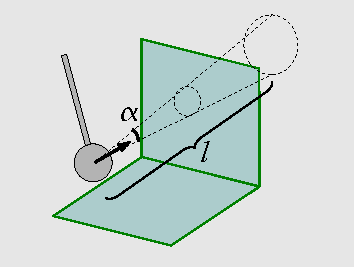
\includegraphics[width=3.4cm]{training}
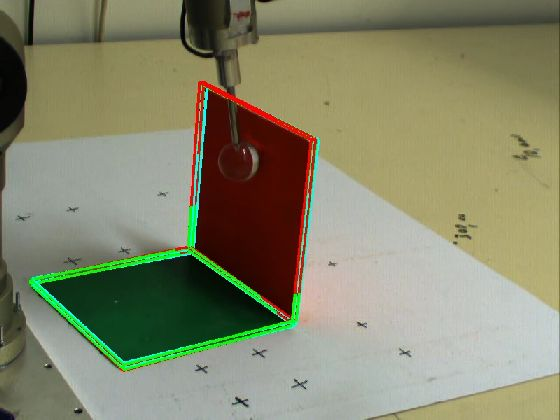
\includegraphics[width=3.4cm]{complex1}
}
\centerline{
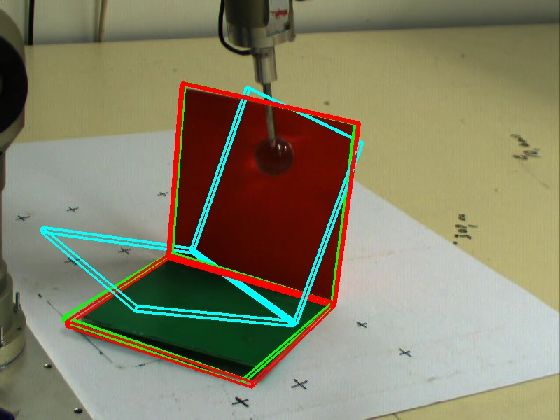
\includegraphics[width=3.4cm]{complex2}
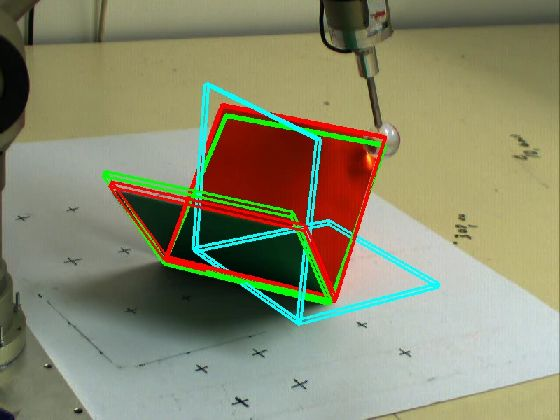
\includegraphics[width=3.4cm]{complex4}
}
\caption[Setup]{
A 5-DOF robotic arm equipped with a finger
performs a random straight-line pushing movement of a
variable length $l$=25$\pm$5 cm within a cone with
angle $\alpha$=20 deg towards an object (top left).
The movement begins at a random location so that every small
region on the upper part of an object is equally likely to be pushed.
%The object behaviour can be complex and varies depending
%on the finger trajectory and its pose relative to the object.
In the image sequence shown above,
%the object begins to rotate anti-clockwise (top right - bottom left)
%before tilting (bottom right).
the red wire-frame shows the output from the vision tracking system,
the green wire-frame indicates the object pose predicted by the
KDEF learning method,
while the blue wire-frame is generated by the PhysX simulator.
%Although the PhysX predictions are qualitatively plausible,
%it was virtually impossible to tune the simulator so that
%its predictions match reality for all training data.
%Note that the entire motion sequence is predicted before the
%physical push is initiated, without any correction from
%visual feedback during the push execution.
}
\label{fig:Setup}
\end{figure}

For real experiments, we used a 5-axis Katana robotic manipulator
 equipped with a single rigid finger.
%and the motion of pushed objects is captured using a
%single camera and a visual tracking algorithm.
Simulation experiments were carried out using the NVIDIA PhysX physics
engine. These simulation experiments provided us
with perfect ground-truth data against which to evaluate predictions,
and also enabled a large number of experiments with different values
of key parameters. Experiments on real objects tested the robustness of
the methods to disturbances and tracking errors. The PhysX engine was
also separately compared to the learning methods when both were
trained or tuned on real data.

%The virtual environment (using NVIDIA PhysX) does not replicate the
%physical properties of the real world perfectly, as is well
%illustrated in Figure~\ref{fig:Setup}. We automatically tuned the
%parameters of the physics engine to best fit the world. However, we
%have found that even when optimised (using variety of numerical
%optimisation techniques, the parameters neither correspond to their
%true values, nor do they generalise. Partly this is because a physics
%engine is a global approximator - when you tune its parameters to
%match one scene, it is unlikely to model a different scene
%well. However, regardless of how well the simulations correspond to
%the real world, the simulations still provide a
%\textit{self-consistent experimental environment} within which to
%compare the accuracy of predictors that have been trained on data
%generated within that environment, while providing perfect
%ground-truth data for training and test motions that are at least
%physically plausible.

Local frames for environment contacts in the -GAE variants were fixed
by hand to the edges of objects. In test cases with new objects the
frames were again fixed by hand.  An item for future work is to
perform this process automatically.  The bandwidth of all
distributions used in the KDE methods, as well as parameters of the
LWPR regression method, were tuned once by hand and kept constant
throughout all the experiments.

Both KDE and LWPR require many parameters to be determined before
learning from a training set.  A model selection procedure was
performed during experiment P1, to establish reasonable values for
these parameters, which were then used in experiments P2 and P3.  It was
not possible to perform fully systematic optimisations due to the size
of the parameter spaces.  Rather, subsets of the parameter space were
selected by inspection and then explored using a grid search.  Models
were evaluated on a hold-out set, distinct from the training set and
the test set. This model selection process was also performed for the
following parameters of the PhysX physics simulator: static friction,
dynamic friction and the coefficient of restitution. Because of the
reduced parameter space we performed grid search for these PhysX
parameters. In addition to model selection the three different
parameterisations (Gauss-Euler, Gauss-Quaternion,
Von-Mises-Fisher-Quat) of rotations for the density estimation method
were studied in experiment P1, and subsequently the best solution was
used in experiments P2 and P3. For LWPR we used the Euler
parameterisation throughout experiments P1, P2 and P3.

For clarity a complete set of acronymns for the algorithm-information
combinations is given in Table~\ref{tab:algs}. The PhysX algorithm has
access to full mesh and contact information when making its
predictions.

\begin{table}[b]
\begin{center}
\begin{tabular}{|l|l|l|l|}\hline
 & \multicolumn{3}{|c|}{Information} \\ \hline
Predictor & G & G+A & G+A+E \\ \hline
LWPR & LWPR-G& LWPR-GA & LWPR-GAE \\ \hline
KDE & KDE-G & KDE-GA & KDE-GAE \\ \hline
KDEF & KDEF-G & KDEF-GA & KDEF-GAE \\ \hline
PhysX & - & - & - \\ \hline
\end{tabular}
\end{center}
\caption{Algorithm-information variants.}
\label{tab:algs}
\end{table}

%%%%%%%%%%%%%%%%%%%%%%%%%%%%%%%%%%%%%%%%%%%%%%%%%%%%%%%%%%%%%%%%%%%%%%%

\subsection{Performance measure}\label{sec:Experiment.Performance}

In all experiments, we took the output of the tracked 6D pose of a
real object to be ground-truth, and compared it against predictions
which were previously forecast by the learned prediction system. The
vision system does not provide perfect ground-truth, yielding typical
errors of around $\pm$2mm during successful tracking, or arbitrarily
large errors during tracking loss. However, comparing
predictions to the outputs of the tracker still provides some useful
information about discrepancies in the predictor, although clearly the
performance of the predictors is limited by the accuracy of the data
on which they are trained. Prediction performance is evaluated as
follows.
\begin{table}[b]
\begin{center}
\begin{tabular}{|l|l|l|l|l|}
\cline{1-4}
Predictor & Polyflap & Box & Cylinder \\
\cline{1-4}
KDEF-G euler & 0.055$\pm$0.002 & 0.061$\pm$0.003 & 0.063$\pm$0.003\\
KDEF-G quat  & \textbf{0.049}$\pm$0.002 & \textbf{0.059}$\pm$0.002 & \textbf{0.059}$\pm$0.003\\
KDEF-G vmf   & 0.057$\pm$0.002 & 0.066$\pm$0.003 & 0.071$\pm$0.003\\
LWPR-G euler &  0.059$\pm$0.002 & 0.118$\pm$0.003 & 0.077$\pm$0.003\\
\cline{1-4}
KDEF-GA euler & 0.054$\pm$0.002 & 0.060$\pm$0.003 & 0.052$\pm$0.002\\
KDEF-GA quat & \textbf{0.044}$\pm$0.002 & \textbf{0.057}$\pm$0.002 & \textbf{0.047}$\pm$0.002\\
KDEF-GA vmf & 0.064$\pm$0.002 & 0.097$\pm$0.002  & 0.109$\pm$0.003 \\
LWPR-GA euler & 0.068$\pm$0.002 & 0.127$\pm$0.003 & 0.105$\pm$0.002 \\
\cline{1-4}
KDEF-GAE euler & 0.083$\pm$0.003 & 0.065$\pm$0.003 & 0.050$\pm$0.002 \\
KDEF-GAE quat & \textbf{0.062}$\pm$0.002 & \textbf{0.065}$\pm$0.003 & \textbf{0.047}$\pm$0.002\\
KDEF-GAE vmf & 0.081$\pm$0.002 & 0.086$\pm$0.002 & 0.065$\pm$0.002\\
LWPR-GAE euler & 0.069$\pm$0.002 & 0.136$\pm$0.003 & 0.116$\pm$0.003\\
\cline{1-4}
KDE-GA euler & 0.053$\pm$0.002 & 0.057$\pm$0.002 & 0.068$\pm$0.003 \\
KDE-GA quat  & \textbf{0.049}$\pm$0.002 & \textbf{0.057}$\pm$0.002 & \textbf{0.065}$\pm$0.003\\
KDE-GA vmf   & 0.062$\pm$0.002 & 0.058$\pm$0.002 & 0.092$\pm$0.004\\
\cline{1-4}
KDE-GAE euler & 0.090$\pm$0.002 & 0.161$\pm$0.003 & 0.071$\pm$0.003\\
KDE-GAE quat  & \textbf{0.087}$\pm$0.002 & 0.253$\pm$0.002 & \textbf{0.068}$\pm$0.003\\
KDE-GAE vmf   & \textbf{0.087}$\pm$0.002 & \textbf{0.127}$\pm$0.003 & 0.091$\pm$0.004\\
\cline{1-4}
PhysX & 0.144$\pm$0.003 &  0.171$\pm$0.003 & 0.271$\pm$0.001\\
\cline{1-4}
\end{tabular}
\end{center}
\caption[Performance Table]{Experiment L: Forward push on a
  polyflap/box/cylinder, trained on real data. Shown is the dimensionless measure normalised average error  ${E_{av}^{norm}} \pm$ standard error.
}\label{tab:PerformanceTableL1av}
\end{table}
At any particular time step, $t$, a large number, $N$, of randomly chosen points $p_{n}^{1,t}$, where $n=1 \ldots N$, are rigidly attached to an object at the ground-truth pose, and the corresponding points $p_{n}^{2,t}$ to an object at the predicted pose. At time step $t$, an average error $E_t$ can now be defined as the mean of displacements between points on the object at the predicted pose and points on the object at the ground-truth pose:
\begin{equation}
E_t = \frac{1}{N} \mathop{\sum}_{n=1 \ldots N}|p_{n}^{2,t}-p_{n}^{1,t}|
\label{eq:defn_Rt}
\end{equation}
Note that for each push action, we predict approximately 150
consecutive steps into the future, with no recursive filtering or
corrector steps, hence it is expected that errors will grow with range
from the initial object pose. We therefore find it more meaningful to
normalise all errors with respect to an ``average range'', $R_t$, of
the object from its starting position, defined as:
\begin{equation}
R_t = \frac{1}{N} \mathop{\sum}_{n=1 \ldots N}|p_{n}^{1,t}-p_{n}^{1,0}|
\label{eq:defn_Et}
\end{equation}
For a test data set, consisting of $K$ robotic pushes, each of which breaks down into many consecutive predictions over $T$ time steps, we can now define average error and normalised average error:
\begin{align}
E_{av} &= \frac{1}{K} \mathop{\sum}_{k=1}^{K} \frac{1}{T} \mathop{\sum}_{t=1}^{T} E_t,
&E_{av}^{norm} &= \frac{1}{K} \mathop{\sum}_{k=1}^{K} \frac{1}{T} \mathop{\sum}_{t=1}^{T} \frac{E_t}{R_t}
\label{eq:Error1}
\end{align}
\noindent Note that this normalised error measure necessarily has no
units.

%\noindent For each set of test data, we also compute final error and normalised final error,
%which represent the typical discrepancy between prediction and ground truth that has accumulated by the end of each full robotic push:

%\begin{subequations}
%\begin{align}
%E_f &= \frac{1}{K} \mathop{\sum}_{k=1}^{K} |p_{n}^{2,T}-p_{n}^{1,T}|, \\
%E_f^{norm} &= \frac{1}{K} \mathop{\sum}_{k=1}^{K} \frac{|p_{n}^{2,T}-p_{n}^{1,T}|}{R_T%}
%\label{eq:Error2}
%\end{align}
%\end{subequations}

%\noindent Note that both normalised errors have no units.

%***SEBASTIAN TO MODIFY THIS PARAGRAPH***:
For experiment P1 we performed 10-fold cross-validation. In each case
we give the size of the training and test sets. The model selection
set was the same size as the test set. For transfer learning
experiments P2 and P3 fixed and disjoint training and test sets were used.

\begin{figure}[t]

\centerline{
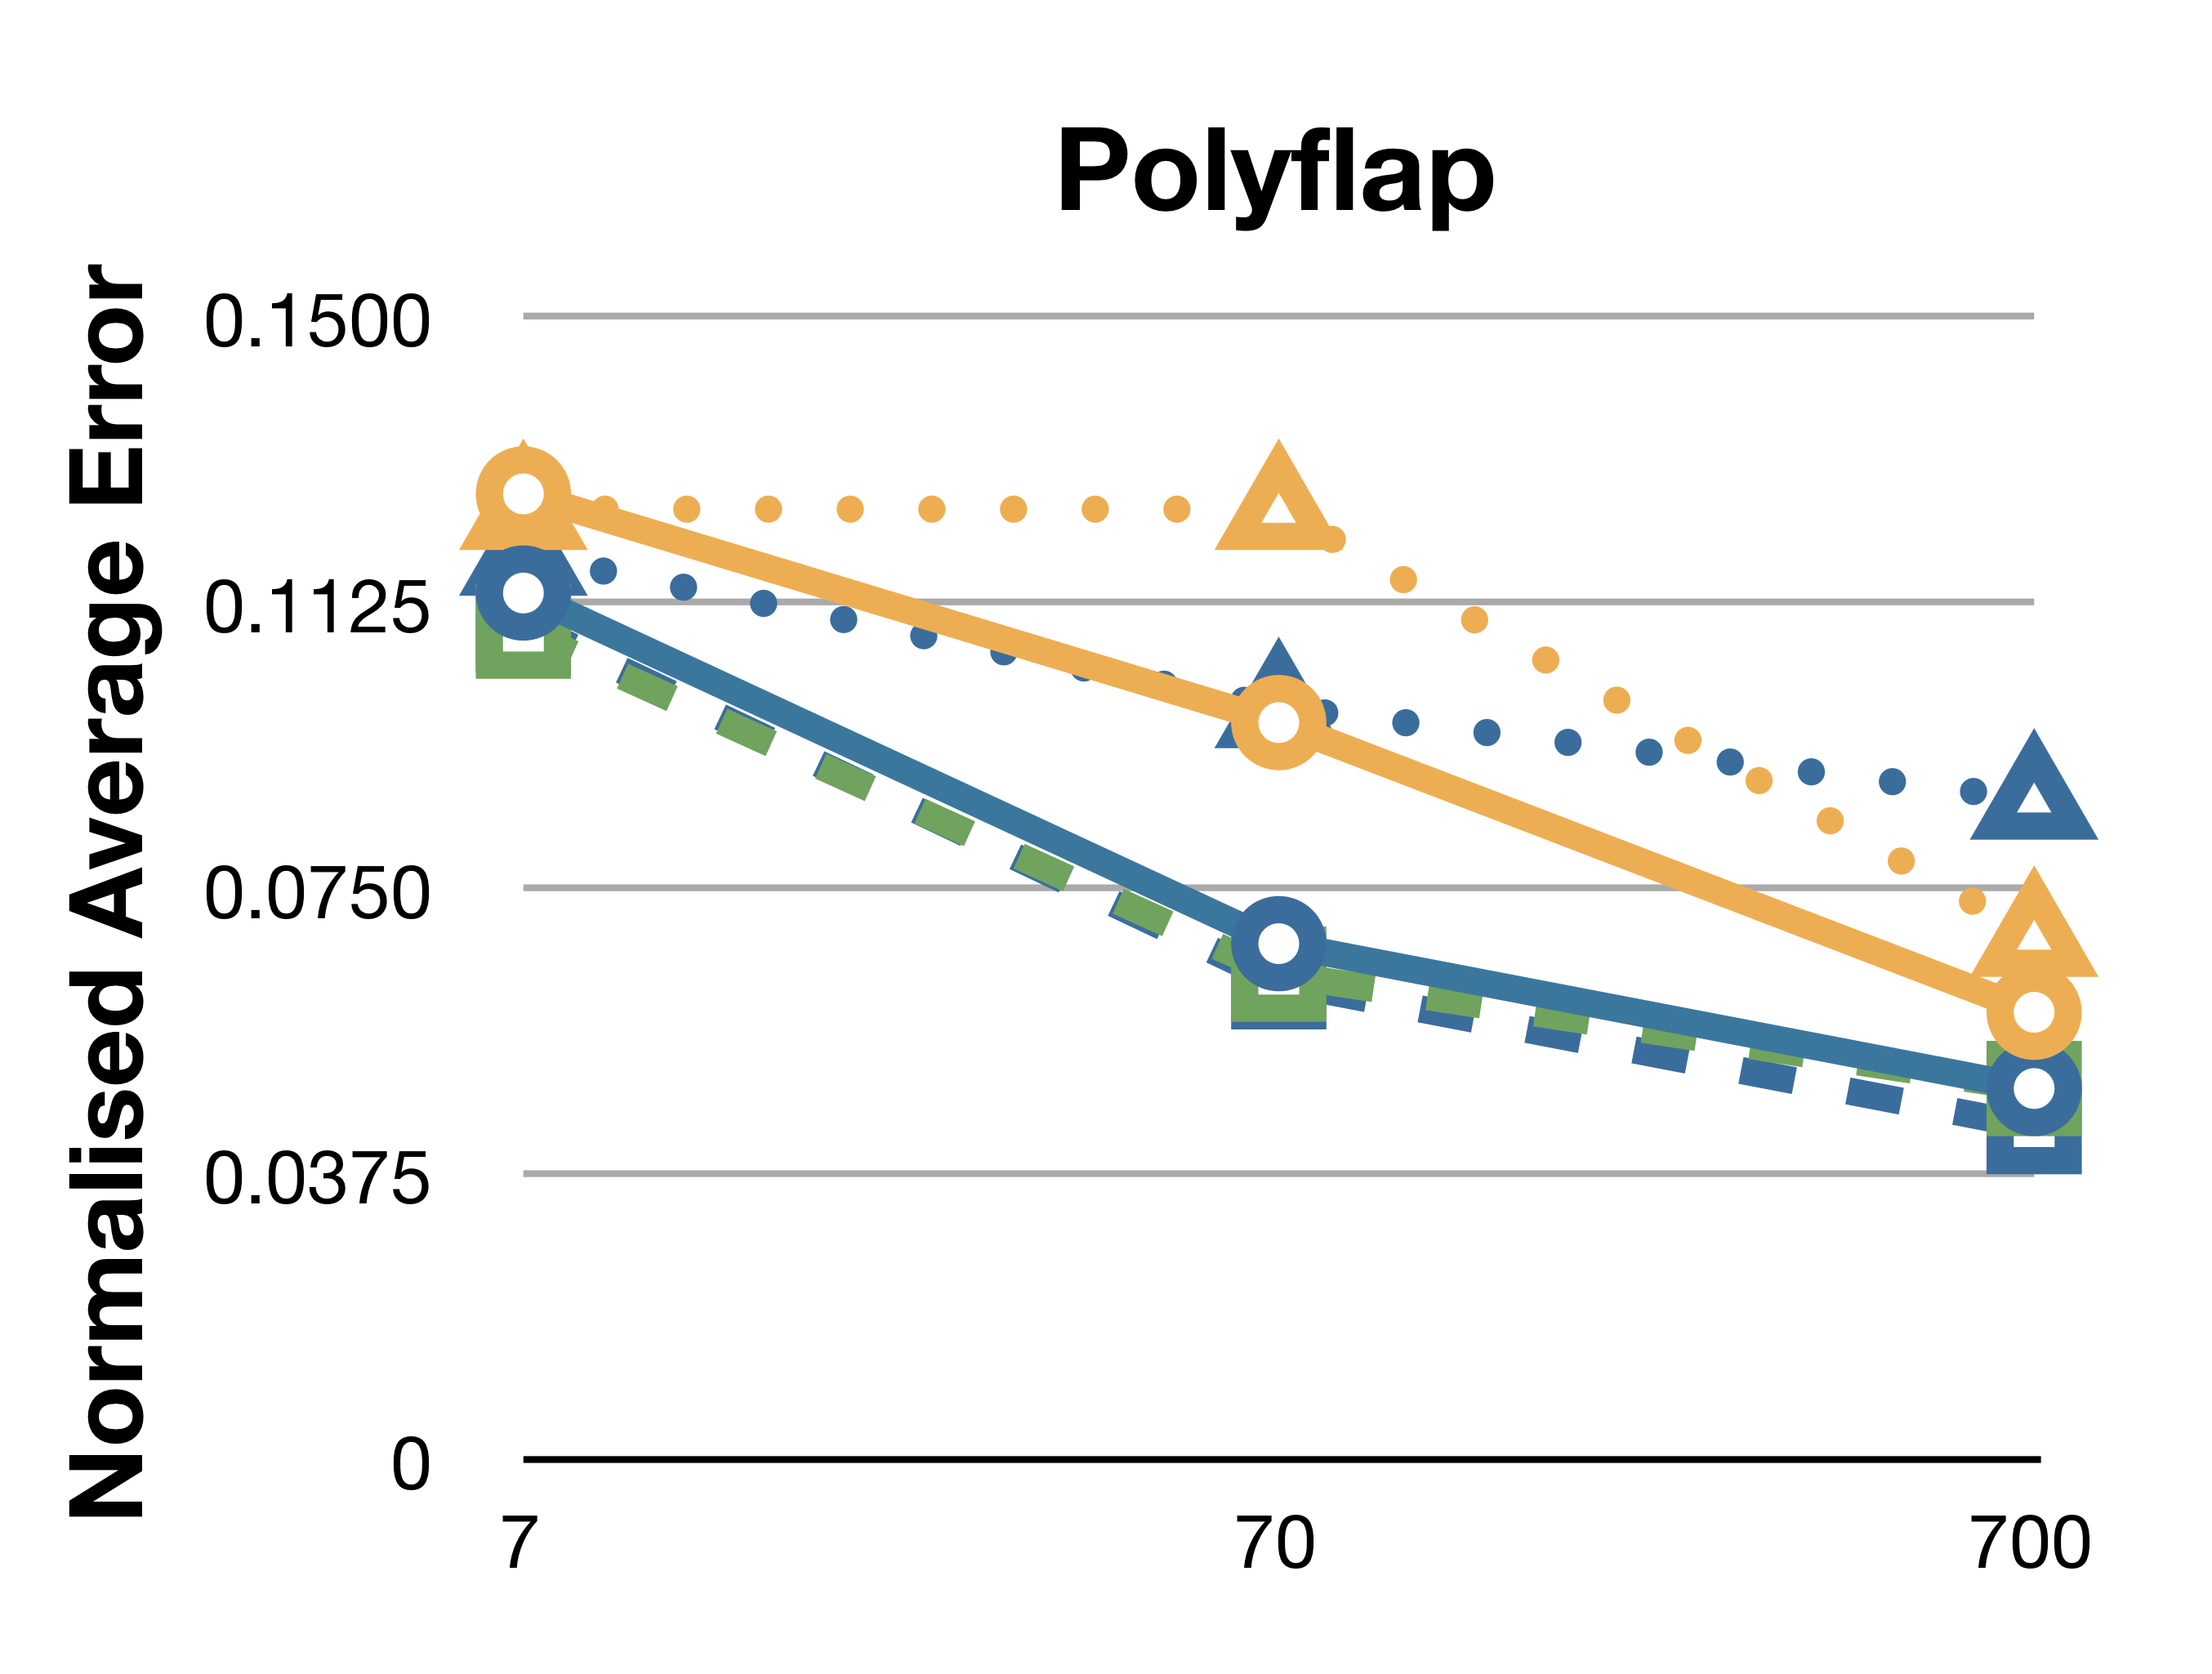
\includegraphics[width=0.45\columnwidth]{graphs_jw/L1av_graph}
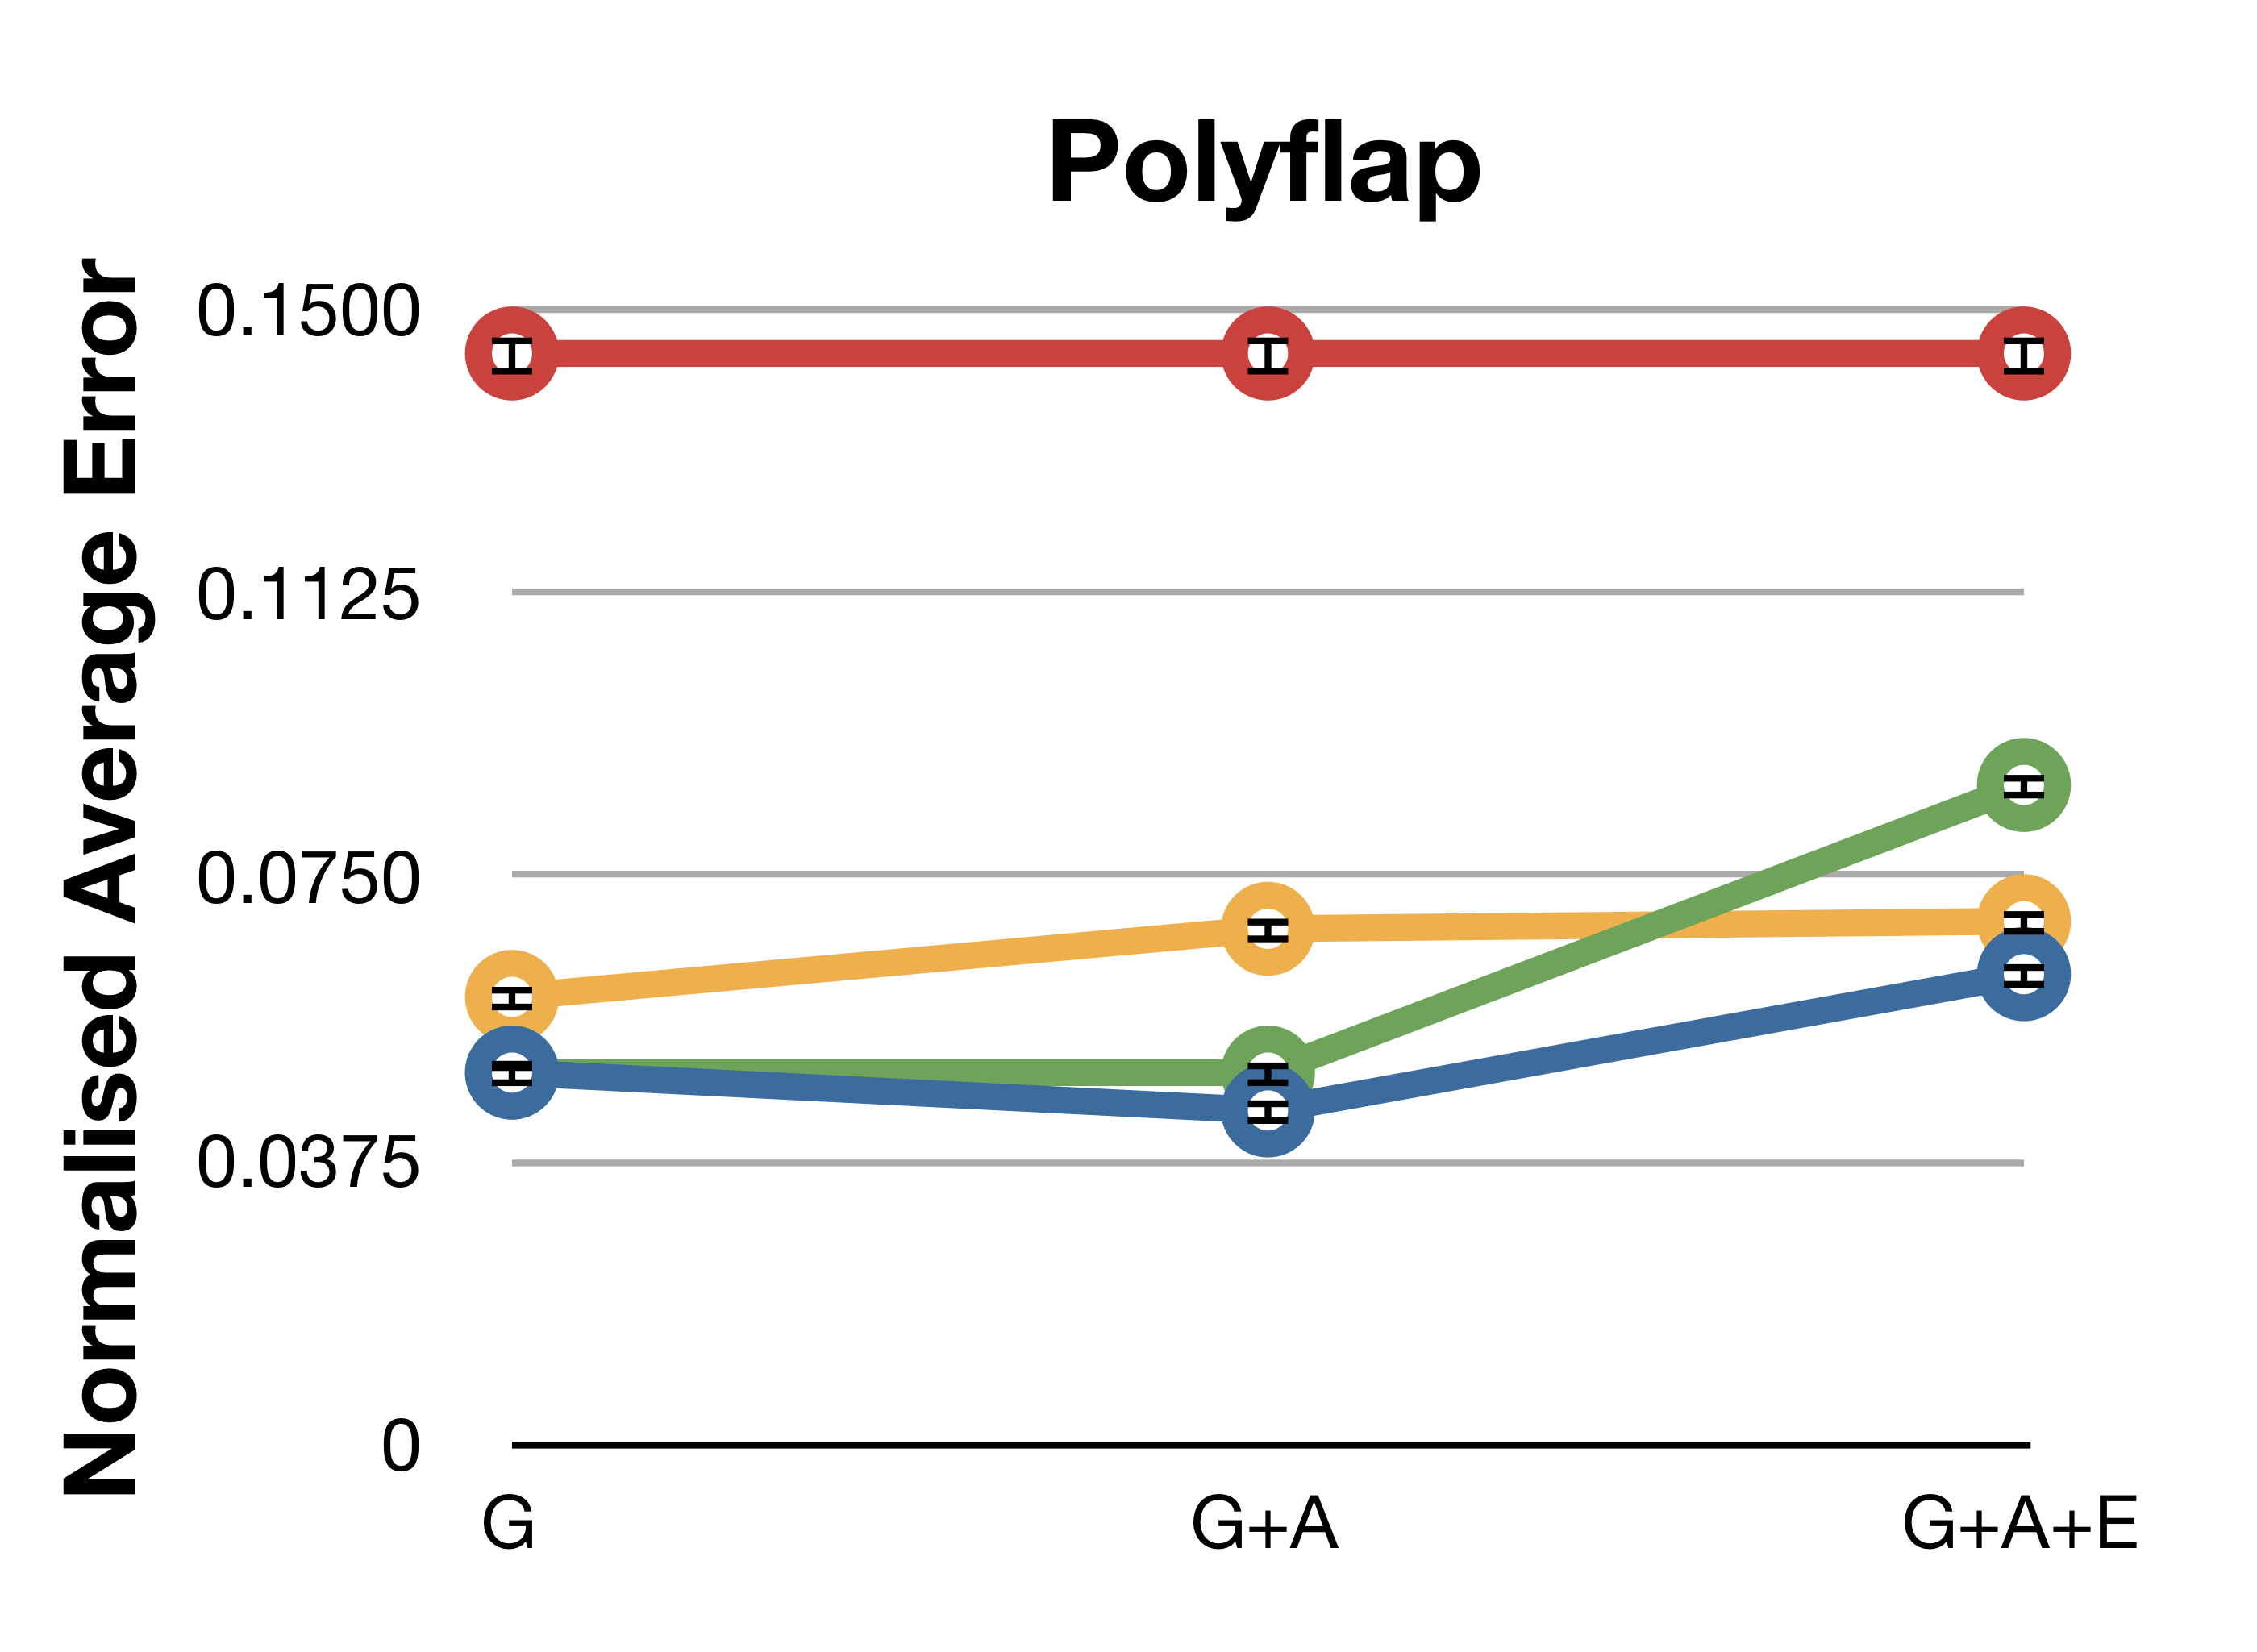
\includegraphics[width=0.45\columnwidth]{graphs_jw/L1av_graph_polyflap}
}

\centerline{
\includegraphics[width=0.45\columnwidth]{graphs_jw/L2av_graph}
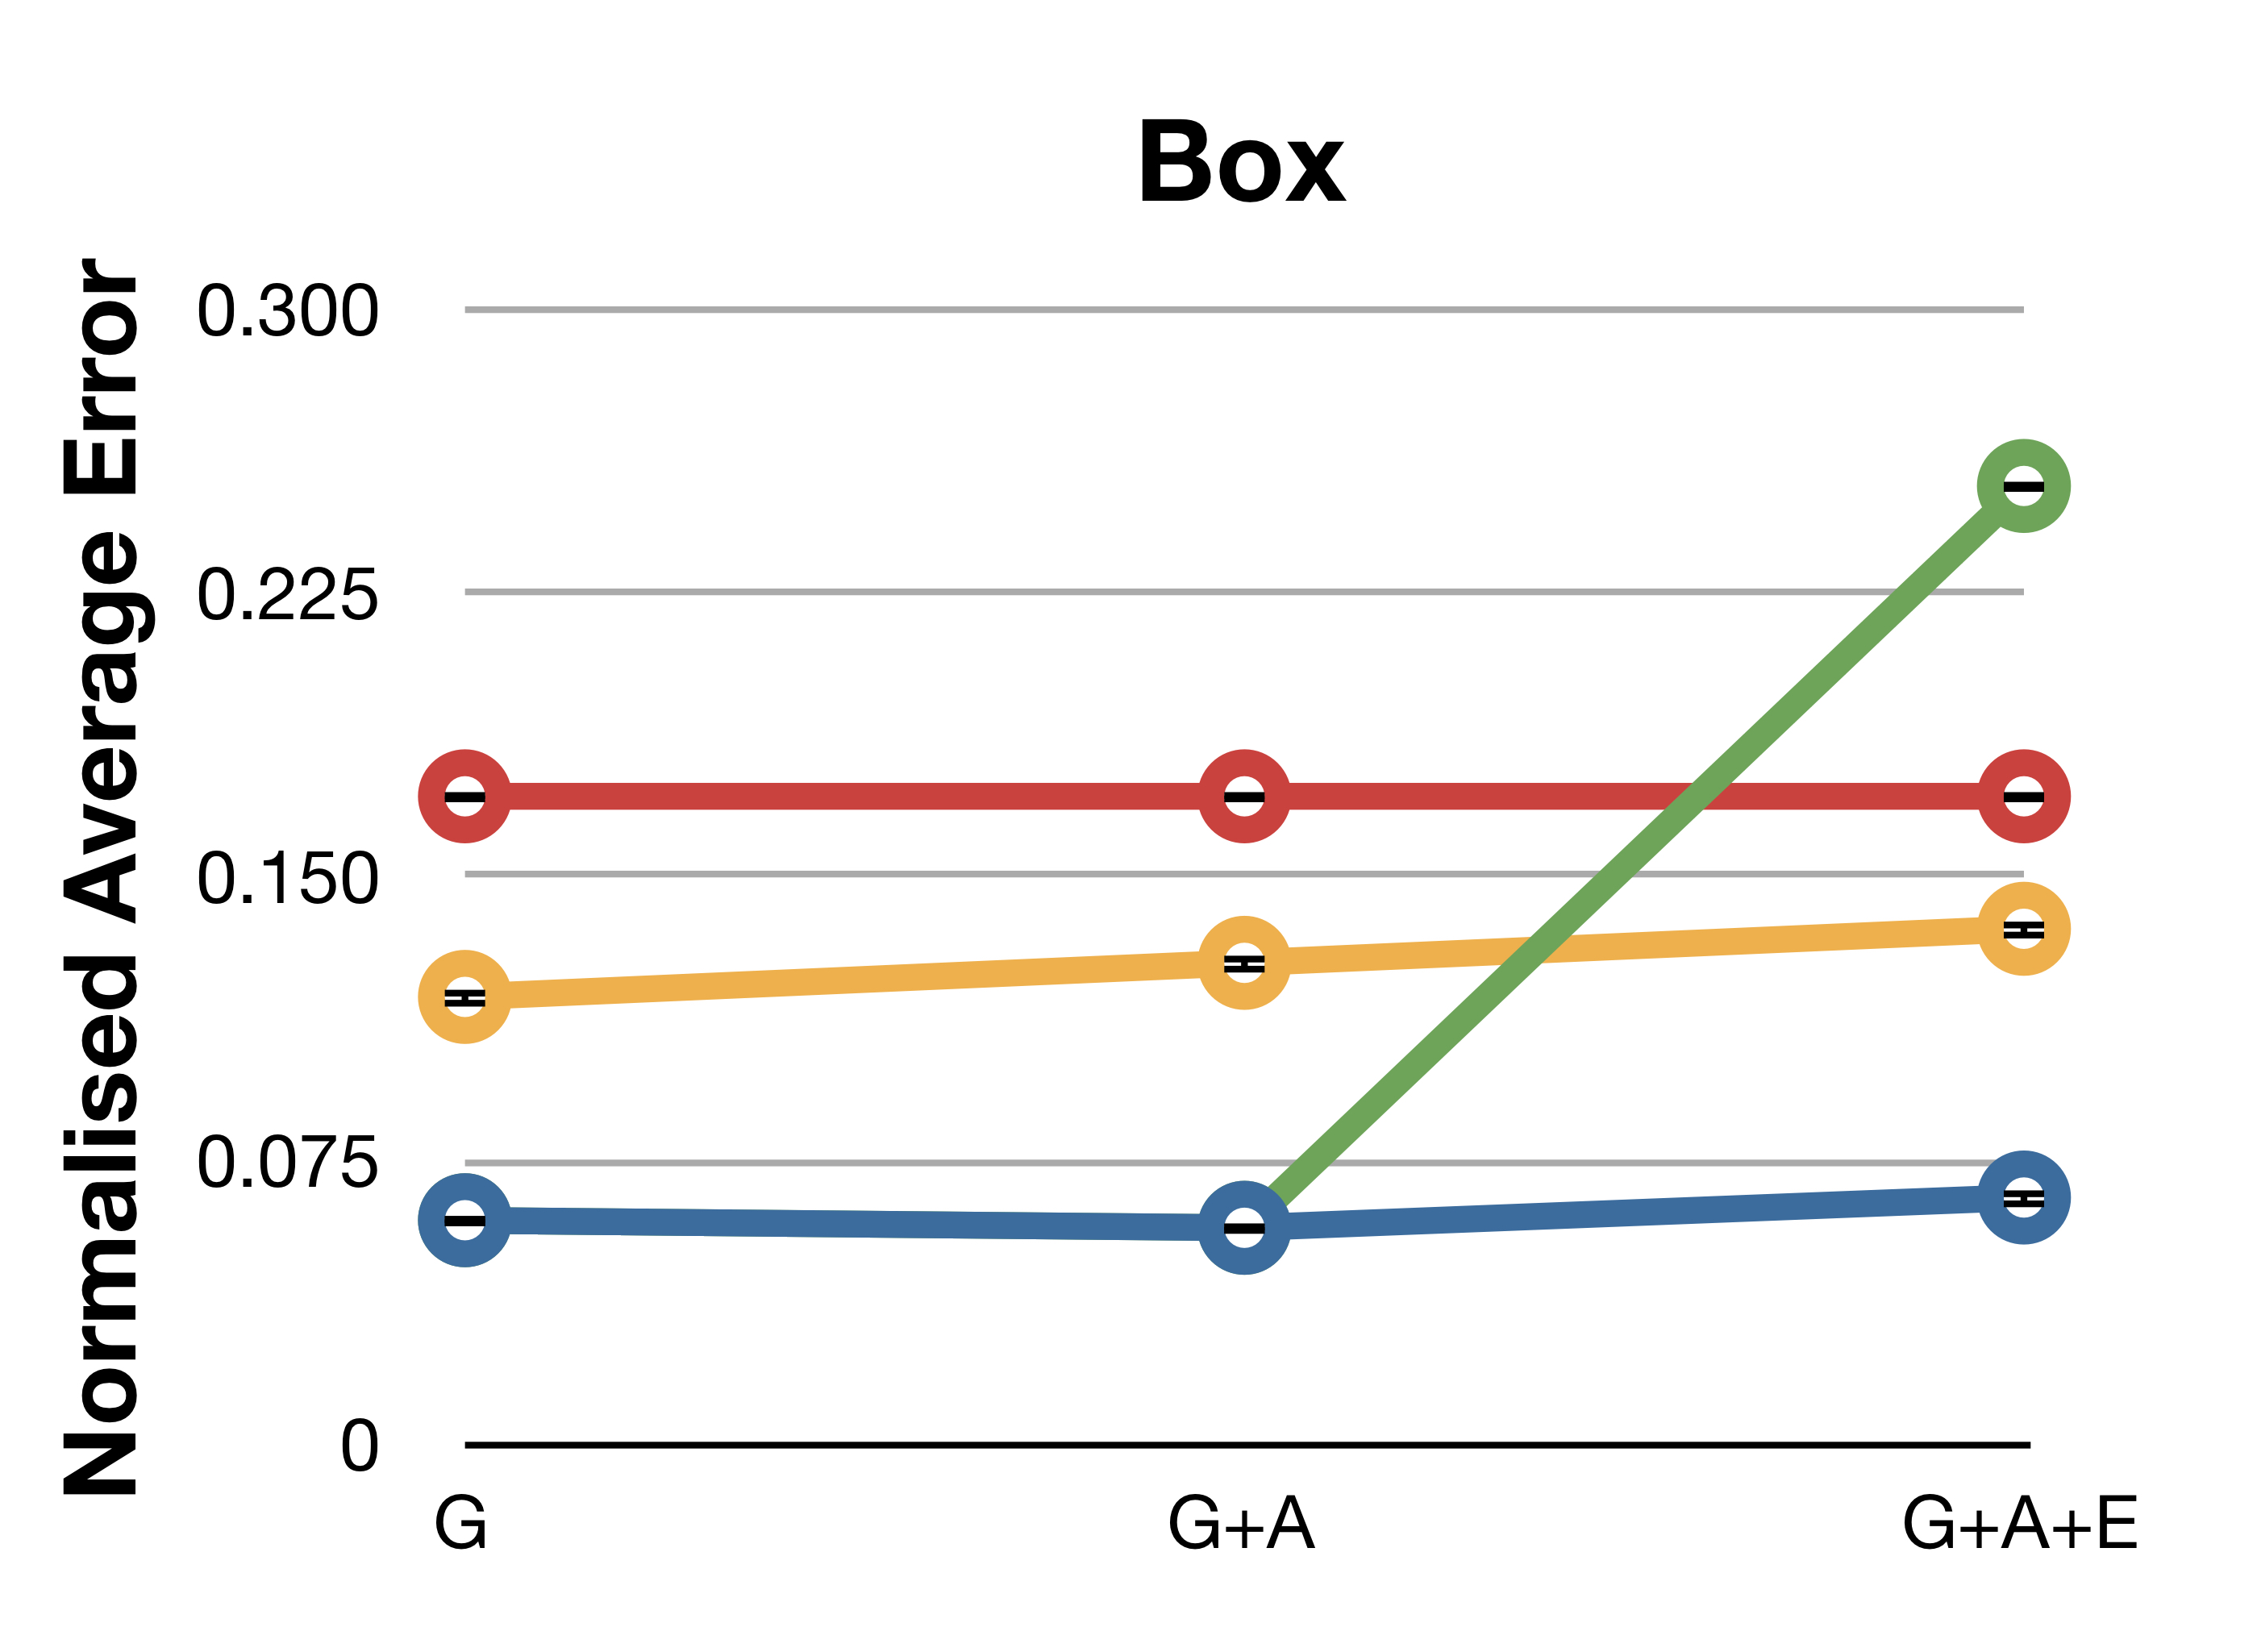
\includegraphics[width=0.45\columnwidth]{graphs_jw/L1av_graph_box}
}

\centerline{\includegraphics[width=0.45\columnwidth]{graphs_jw/L3av_graph}
                 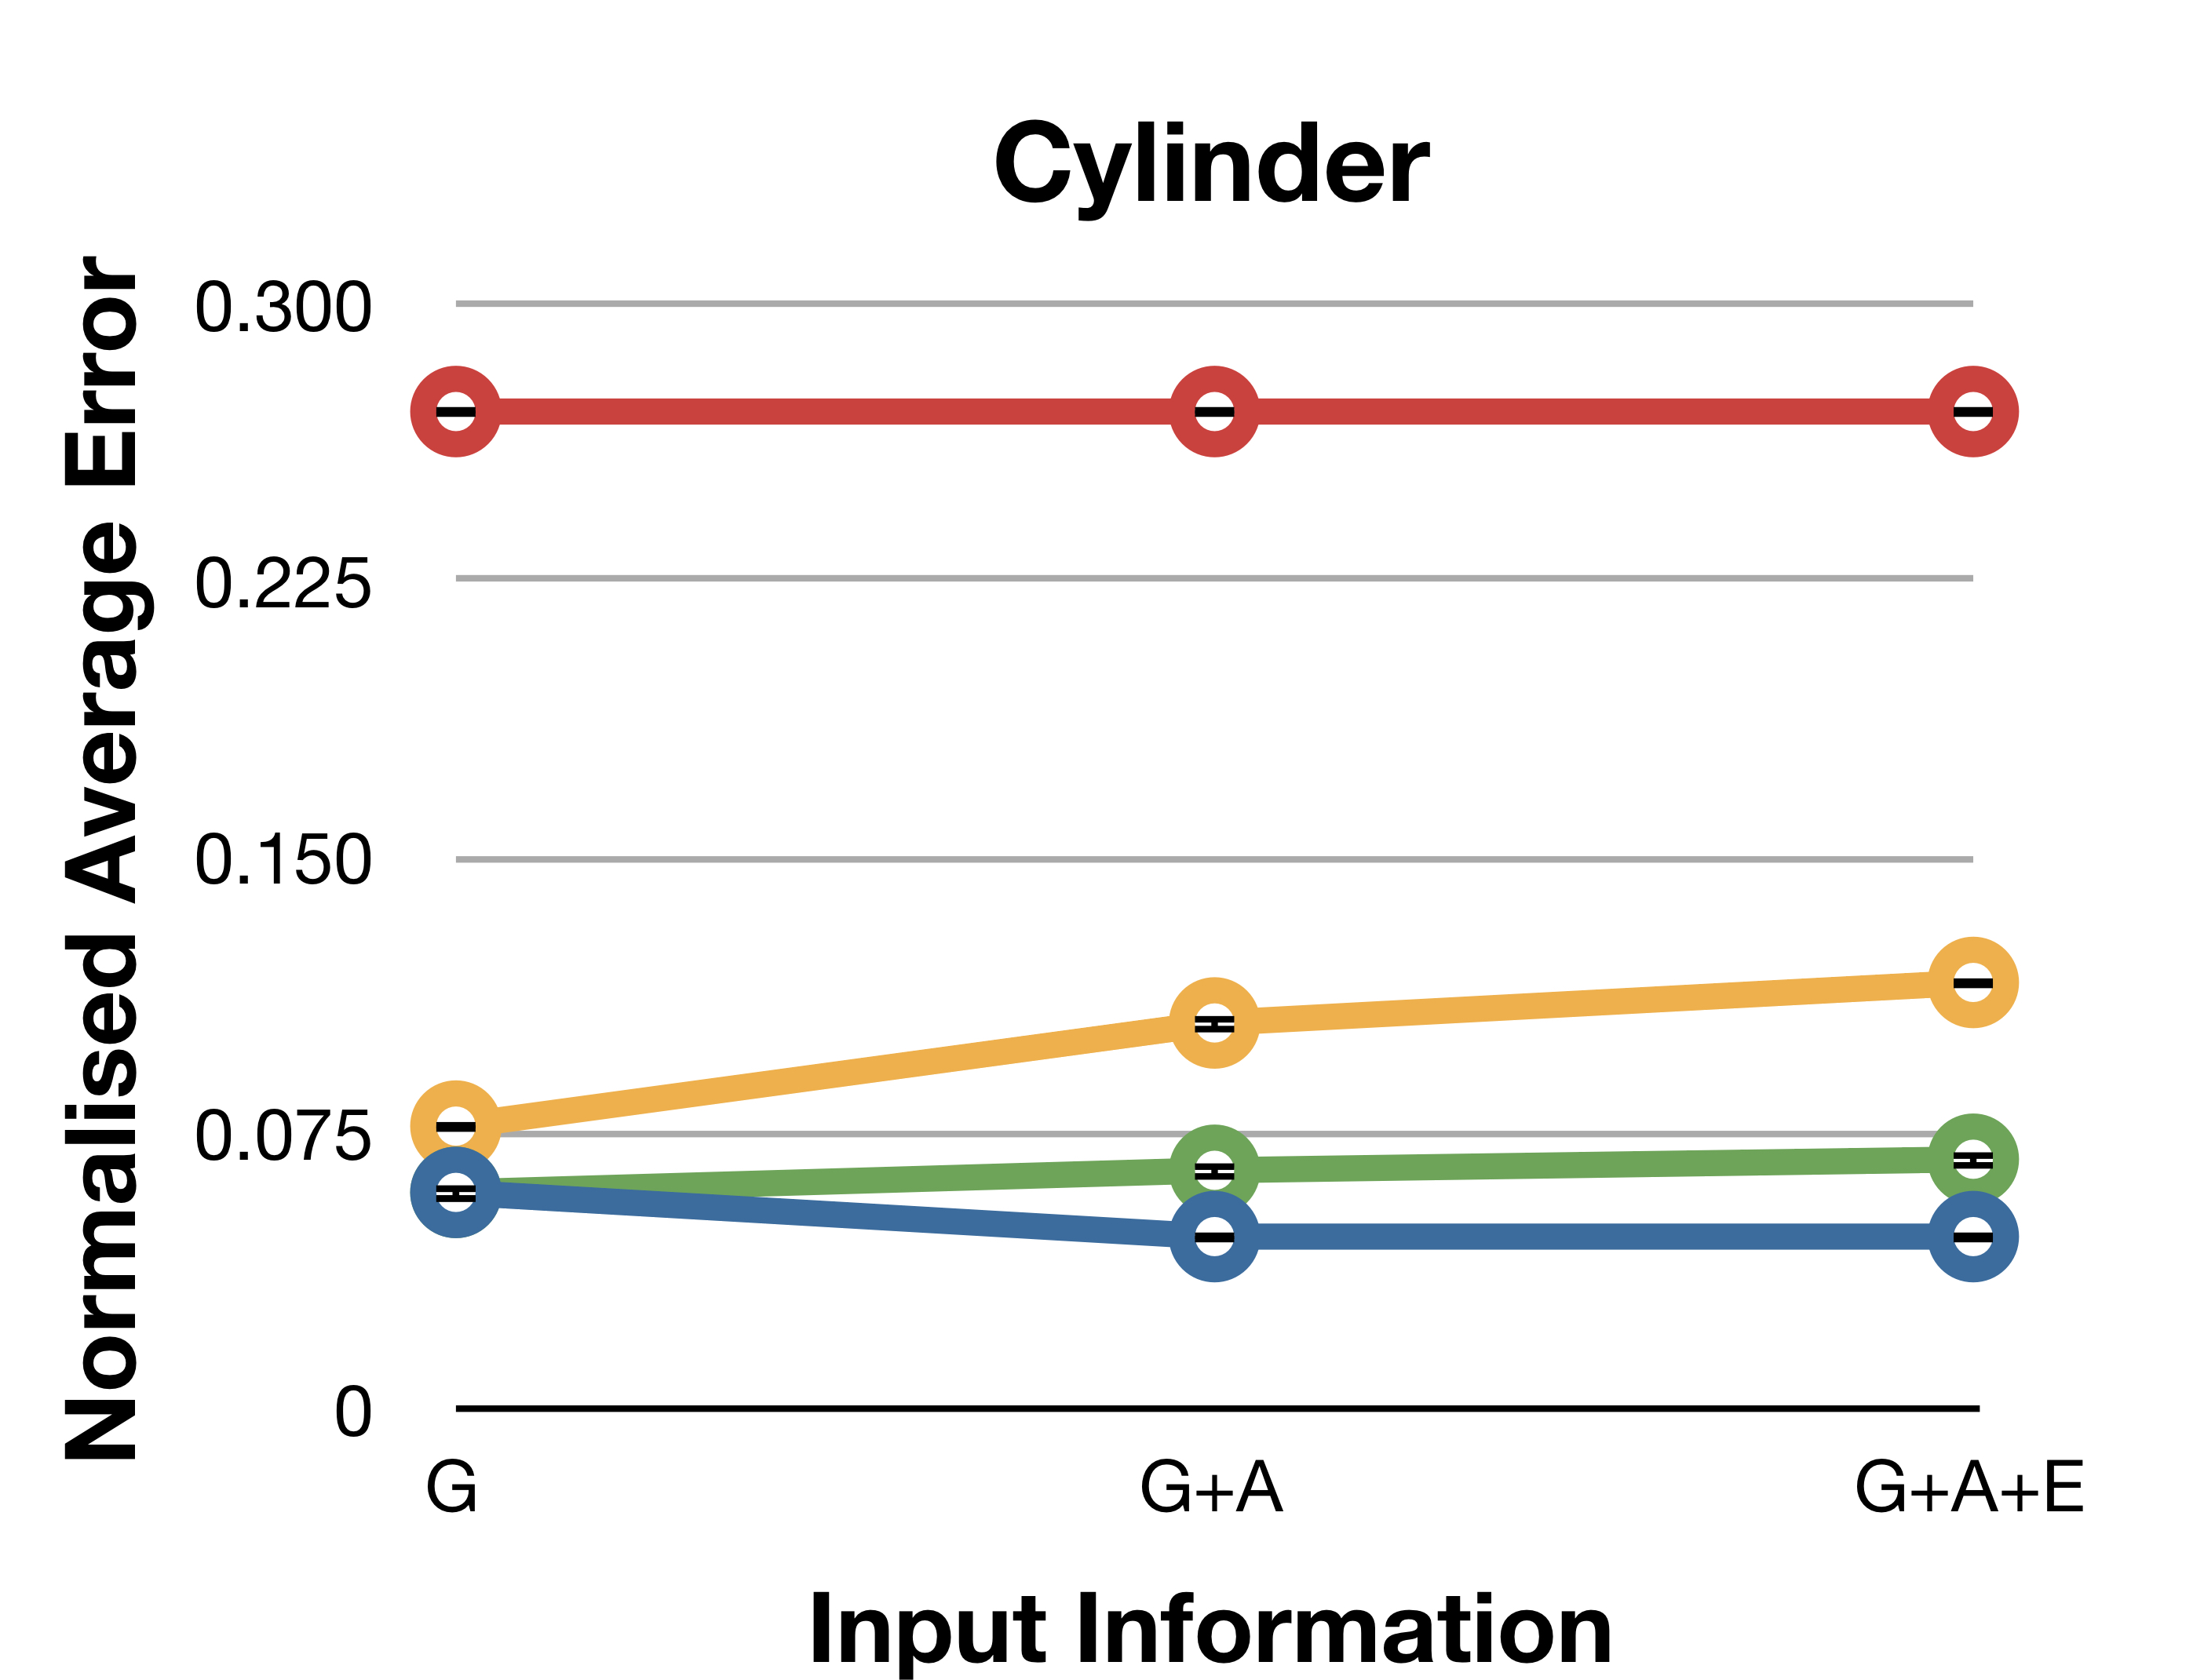
\includegraphics[width=0.45\columnwidth]{graphs_jw/L1av_graph_cylinder}
}
%\vspace{-1mm}
\centerline{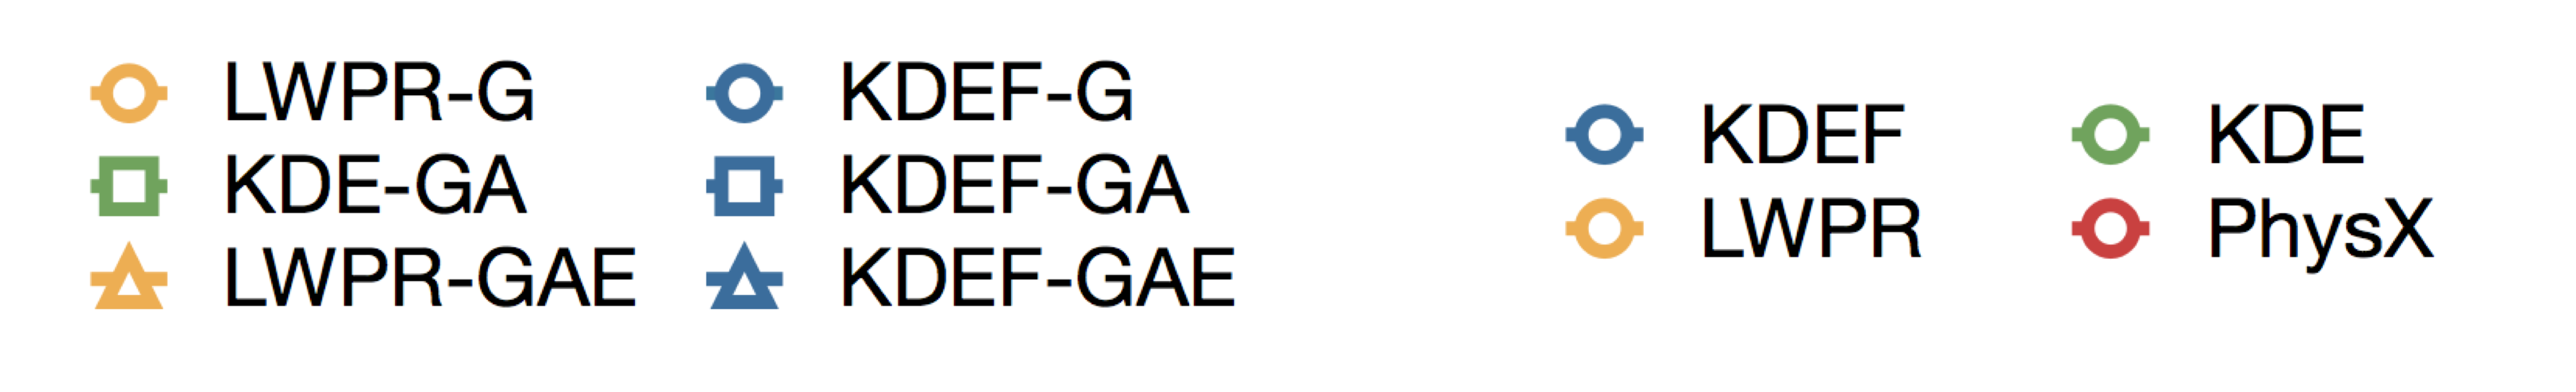
\includegraphics[width=\linewidth]{graphs_jw/L1_convergence_graph_key}}
\vspace{-1mm}
\caption{Experiment P1: Convergence of a selection of learning
  algorithm-information combinations (left column). Change in normalised average prediction
  errors with varying input information (right column). G - global information; A -
  agent-object information; E - object-environment information.}
\label{fig:Lgraphs}
\end{figure}


%%%%%%%%%%%%%%%%%%%%%%%%%%%%%%%%%%%%%%%%%%%%%%%%%%%%%%%%%%%%%%%%%%%%%%%
%%%%%%%%%%%%%%%%%%%%%%%%%%%%%%%%%%%%%%%%%%%%%%%%%%%%%%%%%%%%%%%%%%%%%%%




\section{Results}\label{sec:Results}

\subsection{Experiment P1: Action Interpolation}\label{sec:Results.Learning}

In Experiment P1 the robot applied a set of random pushes to a
polyflap, a box and a cylinder respectively. All the algorithm
variants in Table~\ref{tab:algs} were trained and tested. Model
selection was performed for all algorithm-information combinations as
described previously, including for PhysX. Ten fold cross-validation
was performed for all algorithms. The density estimation techniques
were studied with three parameterisations: Gaussian kernels with 1)
quaternion and 2) Euler angle $SO(3)$ parameterisations as well as 3)
von Mises-Fisher kernels. Training (and testing) sets were 200 (25)
pushes (cylinder), 400 (50) pushes (box) and 700 (90) pushes
(polyflap). Convergence of the best performing learning algorithms
with increasing amounts of data is shown in Figure~\ref{fig:Lgraphs}
(left column). 
%Table~\ref{tab:PerformanceTableL1av} shows the
%generalisation performance after training for each object, and how
%this varies with the parameterisation method.
 Figure~\ref{fig:Lgraphs} (right column) shows how performance varies with input information about contacts for the best versions of all the algorithms.  Table~\ref{tab:PerformanceTableL1av} shows the results of model selection on the different parameterisations for KDE. Image sequences of predicted vs actual trajectories are shown in (Figure~\ref{fig:ExperimentL2}).

\newlength{\imgAXwid}
\setlength{\imgAXwid}{2.15cm}

%\begin{figure}[t]
%\centerline{
%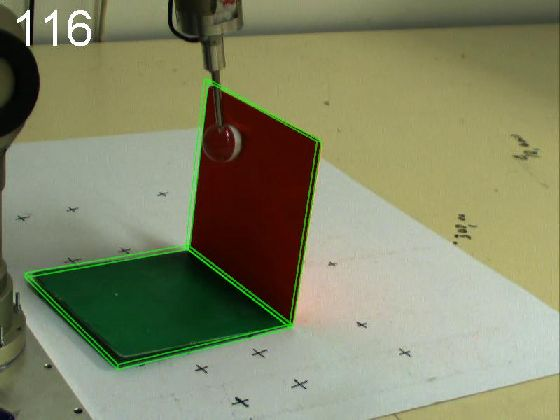
\includegraphics[width=\imgAXwid]{images/A1_2exp_402_1}
%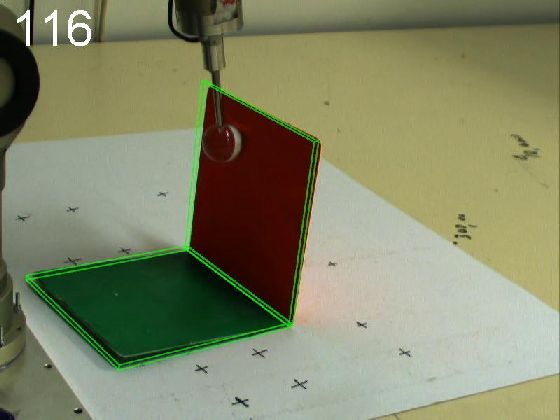
\includegraphics[width=\imgAXwid]{images/A1_LWPR1_402_1}
%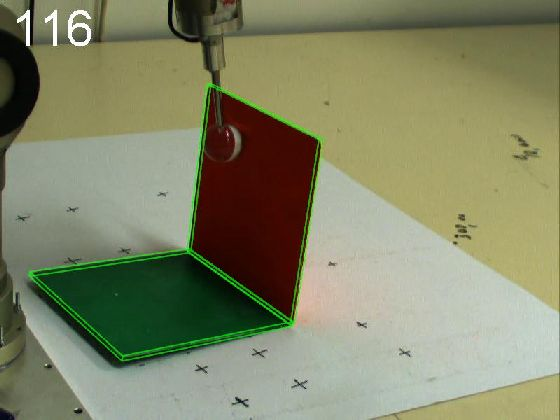
\includegraphics[width=\imgAXwid]{images/A1_physx_402_1}
%}
%%\vspace{0.1cm}
%\centerline{
%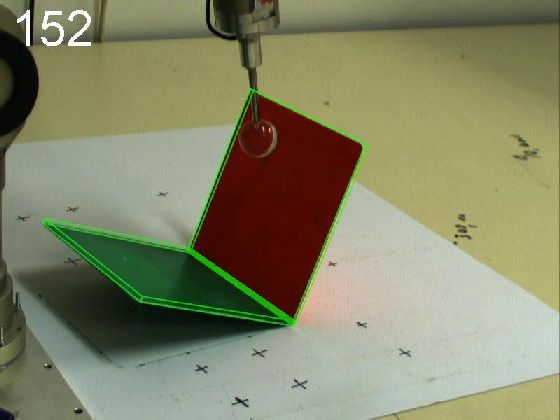
\includegraphics[width=\imgAXwid]{images/A1_2exp_402_2}
%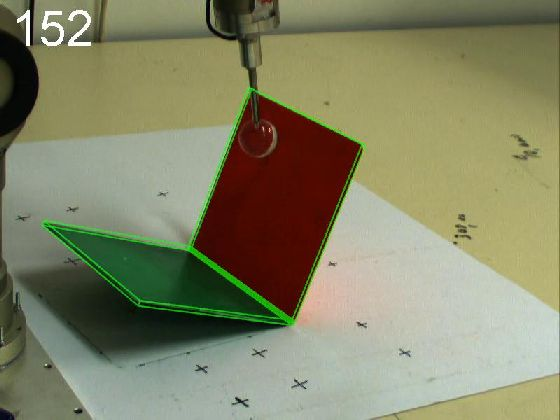
\includegraphics[width=\imgAXwid]{images/A1_LWPR1_402_2}
%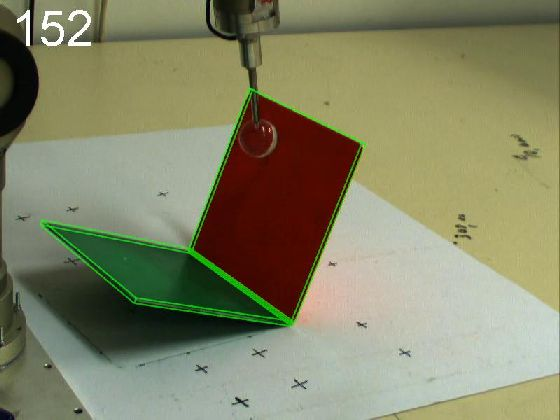
\includegraphics[width=\imgAXwid]{images/A1_physx_402_2}
%}
%%\vspace{0.1cm}
%\centerline{
%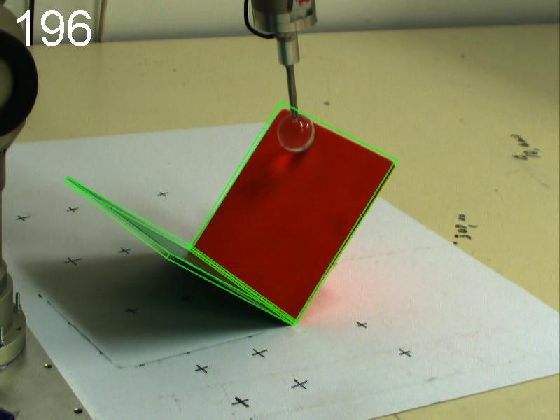
\includegraphics[width=\imgAXwid]{images/A1_2exp_402_3}
%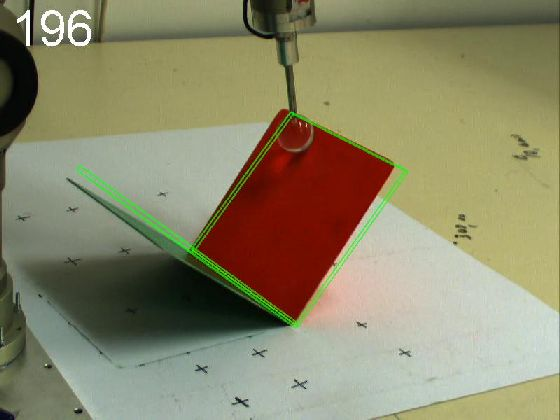
\includegraphics[width=\imgAXwid]{images/A1_LWPR1_402_3}
%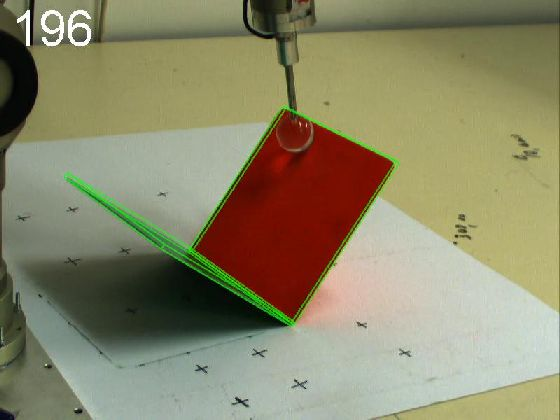
\includegraphics[width=\imgAXwid]{images/A1_physx_402_3}
%}
%%\vspace{0.1cm}
%\centerline{
%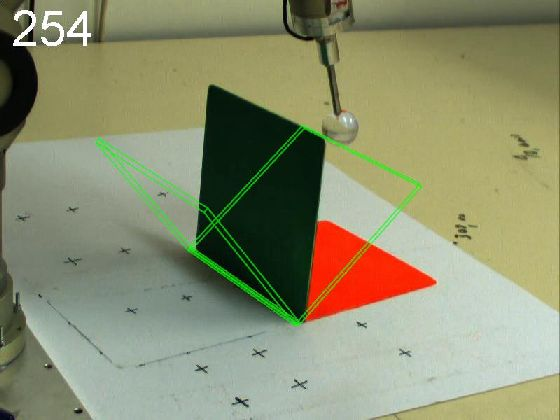
\includegraphics[width=\imgAXwid]{images/A1_2exp_402_4}
%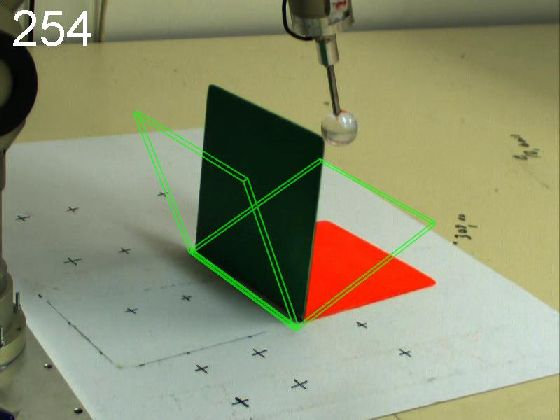
\includegraphics[width=\imgAXwid]{images/A1_LWPR1_402_4}
%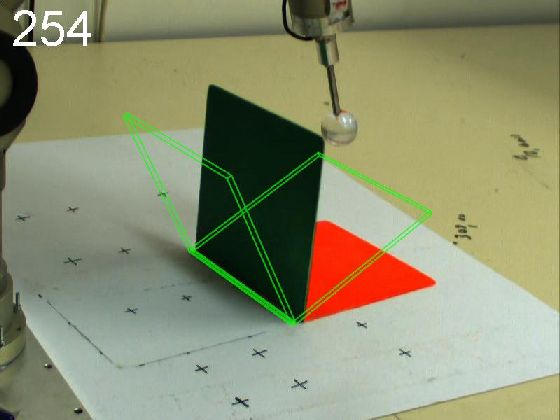
\includegraphics[width=\imgAXwid]{images/A1_physx_402_4}
%}
%%\vspace{0.1cm}
%\centerline{
%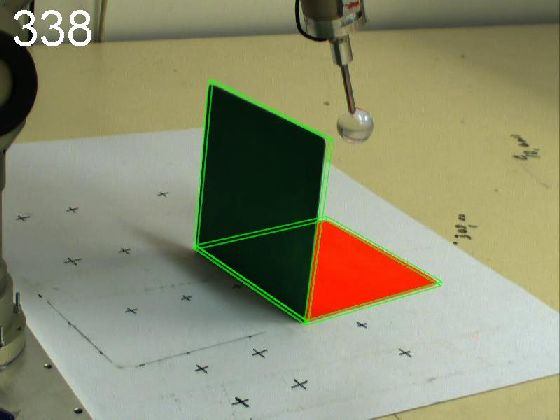
\includegraphics[width=\imgAXwid]{images/A1_2exp_402_5}
%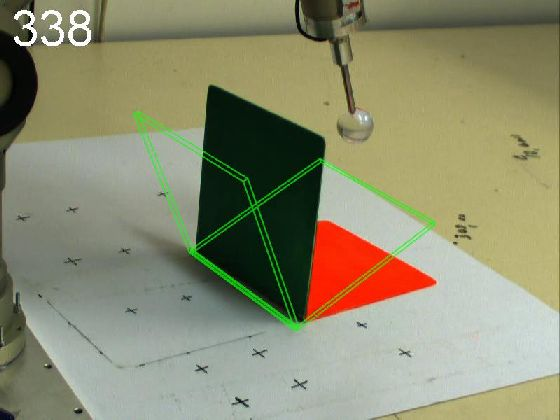
\includegraphics[width=\imgAXwid]{images/A1_LWPR1_402_5}
%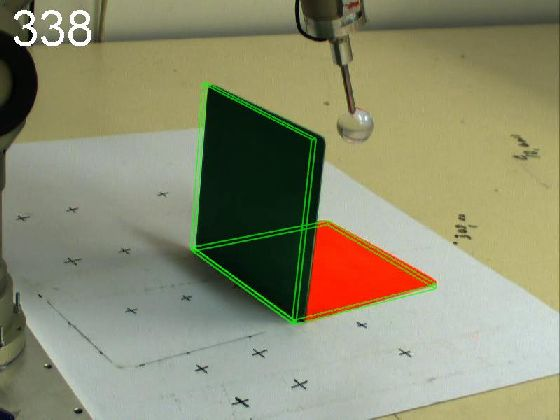
\includegraphics[width=\imgAXwid]{images/A1_physx_402_5}
%}
%\caption {Experiment L: polyflap. Green outline shows the predictions
%  (from left column to right column) by KDEF-GA/quat, LWPR-G, and PhysX for
%  the same trial. Note that LWPR-G doesn't predict the final fall of
%  the polyflap (The frame number is shown in
%  the top left of each image.)  }
%\label{fig:ExperimentL1}
%\end{figure}


%\begin{figure}[t]
%\begin{center}%{\bf Polyflap   \hspace{3cm}        Box} \\
%\centerline{ 
%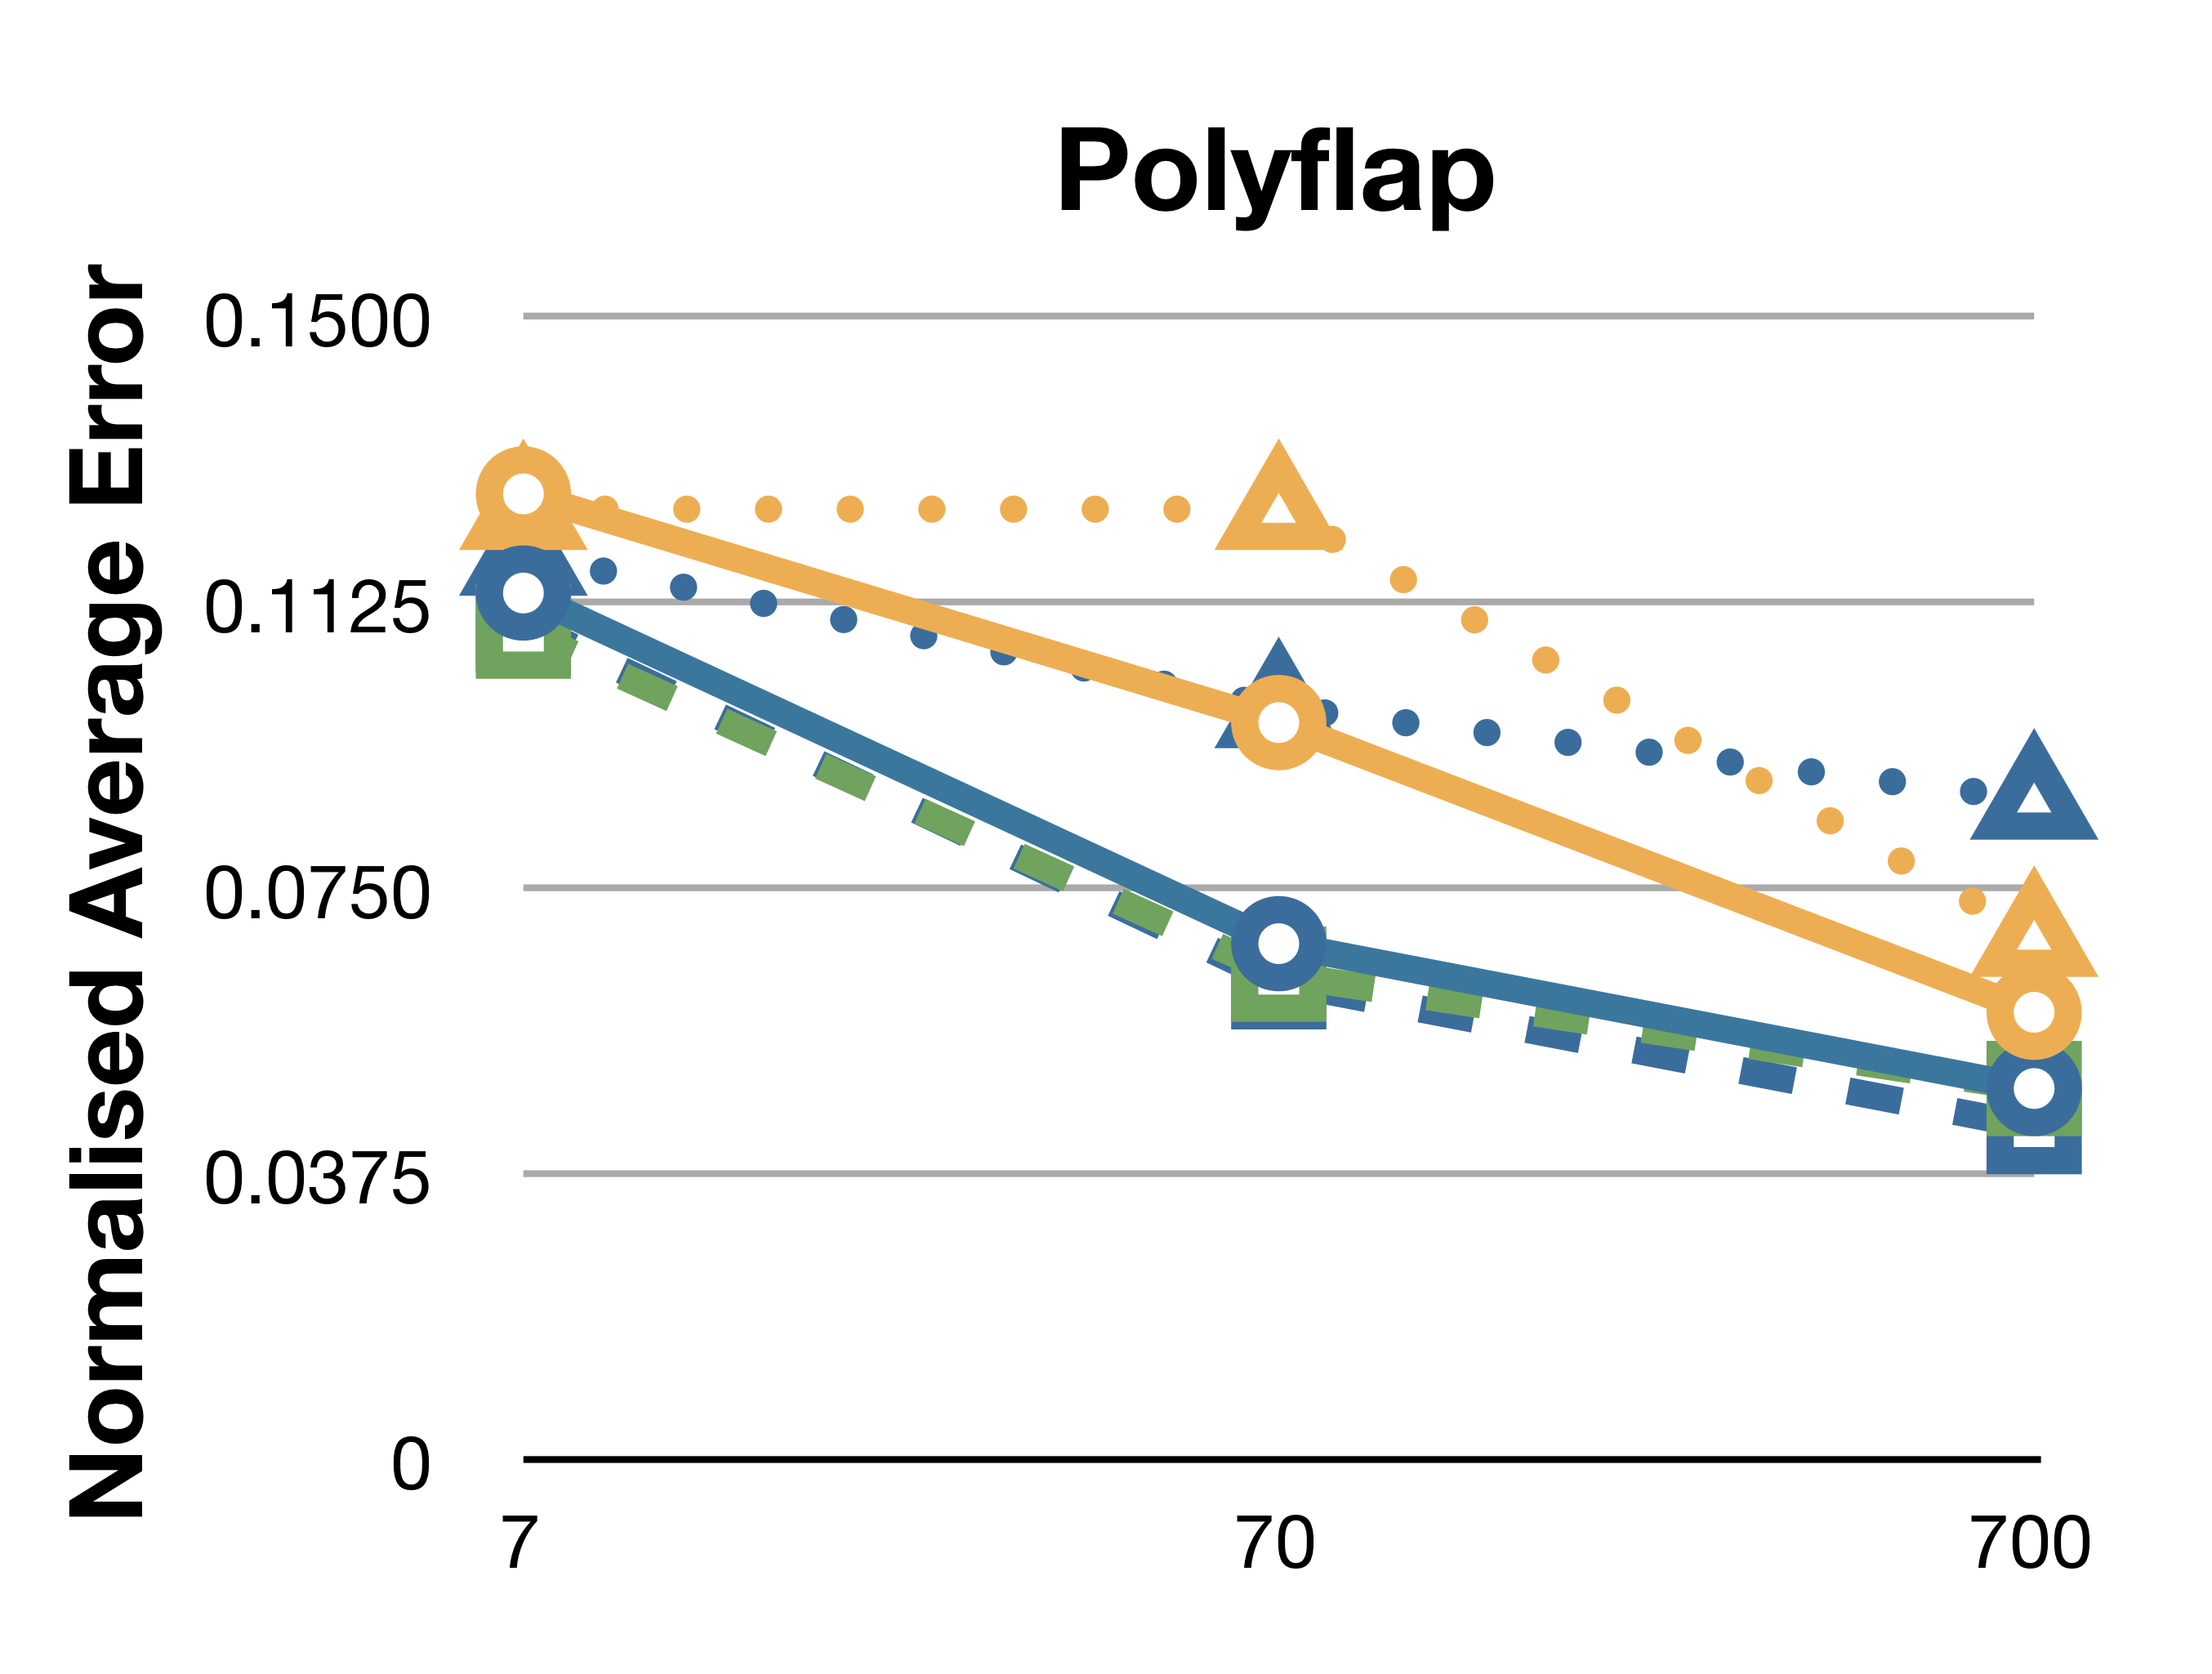
\includegraphics[width=4.5cm]{graphs_jw/L1av_graph}
%\includegraphics[width=4.5cm]{L1final_graph}
%} 
 %{\bf Box} \\
%\centerline{
%\includegraphics[width=4.5cm]{graphs_jw/L2av_graph}
%\includegraphics[width=4.5cm]{L2final_graph}
%}
%{\bf Cylinder}\\
%\centerline{
%\includegraphics[width=4.5cm]{graphs_jw/L3av_graph}
%\includegraphics[width=4.5cm]{L3final_graph}
%}
%\end{center}
%\caption{Experiment L: Convergence of a selection of learning
%  algorithm-information combinations. Data was from pushes on a
%  polyflap, box, and cylinder. All algorithms were trained and tested
%  on real data. Graphs show the decrease in average normalised
%  prediction error with an increasing number of learning trials.}
%\label{fig:Lgraphs}
%\end{figure}




%\begin{figure}[htbp]
%\centerline{
%\includegraphics[width=4.5cm]{L2av_graph}
%\includegraphics[width=4.5cm]{L2final_graph}
%}
%\caption{Experiment L2: forward push on a box, trained and tested on real data. Decrease in average (left) and% final (right) prediction errors with increasing number of learning trials.
%LWPR-G performance versus KDEF with varying input information.}
%\label{fig:L2graphs}
%\end{figure}


%\begin{figure}[htbp]
%\centerline{
%\includegraphics[width=4.5cm]{L3av_graph}
%\includegraphics[width=4.5cm]{L3final_graph}
%}
%\caption{Experiment L3: forward push on a cylinder, trained and tested on real data. Decrease in average (left) and final (right) prediction errors with increasing number of learning trials.
%LWPR-G performance versus KDEF with varying input information.}
%\label{fig:L3graphs}
%\end{figure}





% \begin{figure*}[htbp]
% \centerline{
% 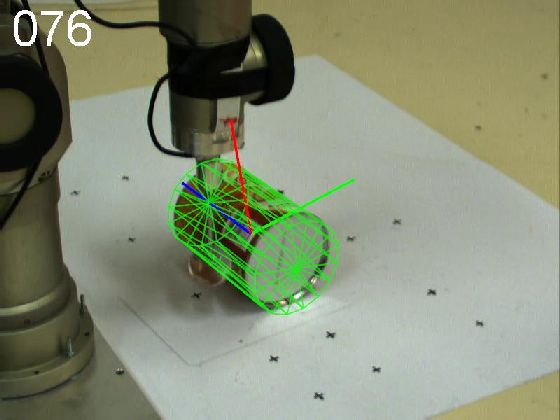
\includegraphics[width=2.3cm]{images/A3_2exp_39_1}
% 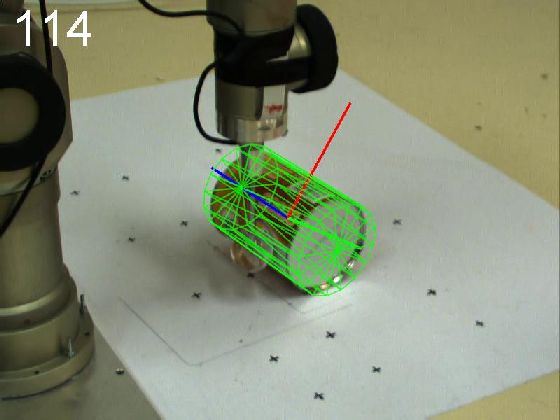
\includegraphics[width=2.3cm]{images/A3_2exp_39_2}
% 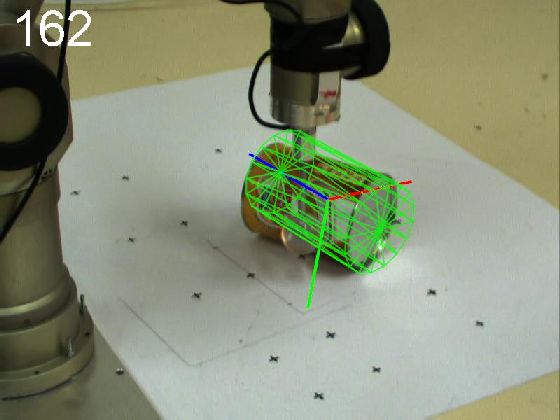
\includegraphics[width=2.3cm]{images/A3_2exp_39_3}
% 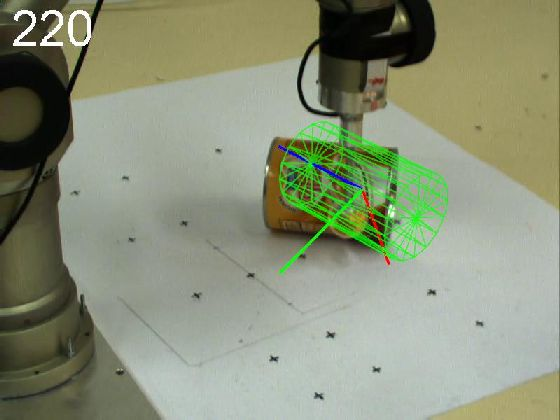
\includegraphics[width=2.3cm]{images/A3_2exp_39_4}
% 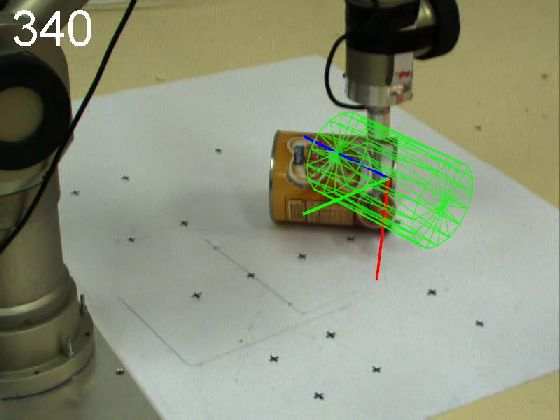
\includegraphics[width=2.3cm]{images/A3_2exp_39_5}
% }
% \vspace{0.1cm}
% \centerline{
% 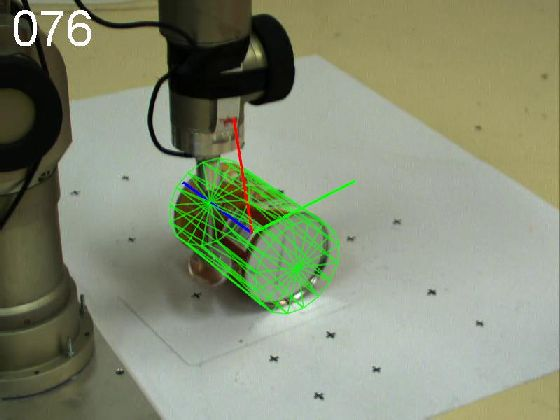
\includegraphics[width=2.3cm]{images/A3_LWPR1_39_1}
% 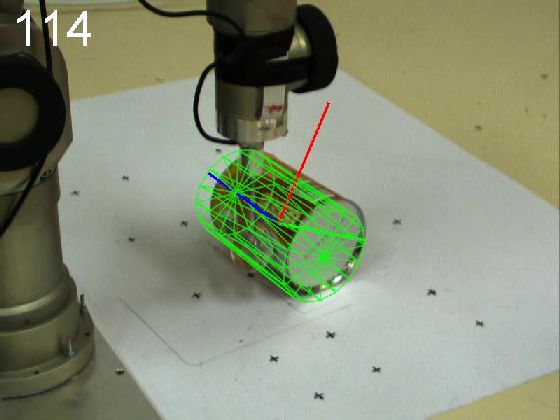
\includegraphics[width=2.3cm]{images/A3_LWPR1_39_2}
% 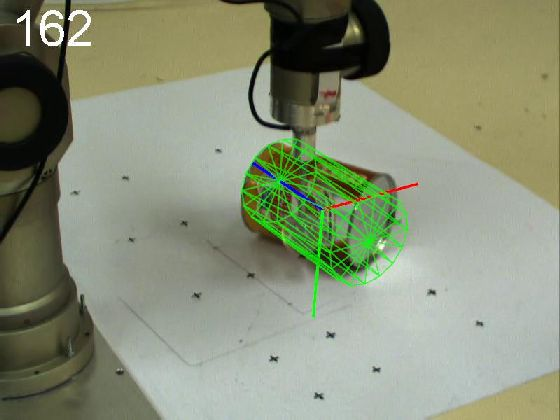
\includegraphics[width=2.3cm]{images/A3_LWPR1_39_3}
% 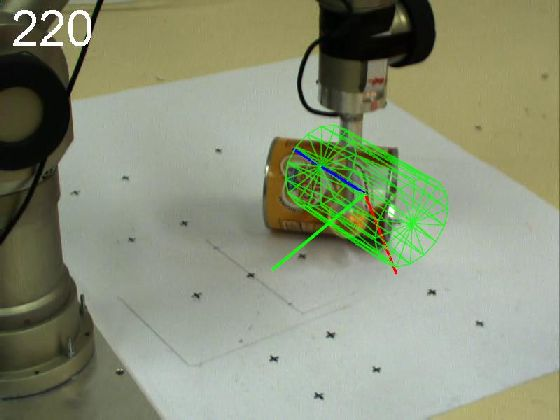
\includegraphics[width=2.3cm]{images/A3_LWPR1_39_4}
% 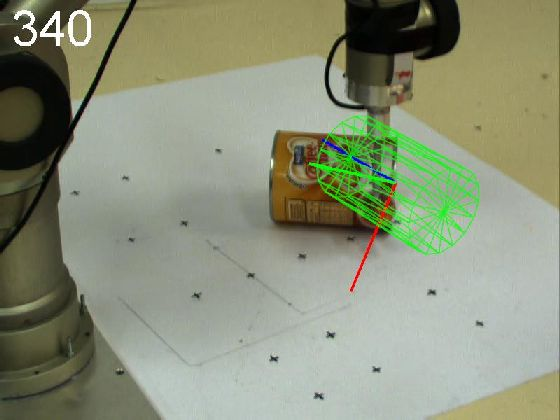
\includegraphics[width=2.3cm]{images/A3_LWPR1_39_5}
% }
% \vspace{0.1cm}
% \centerline{
% 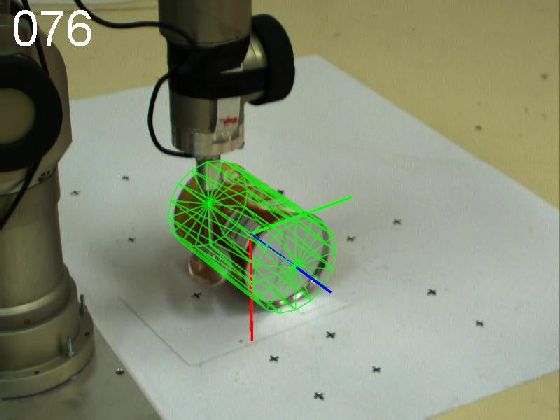
\includegraphics[width=2.3cm]{images/A3_physx_39_1}
% 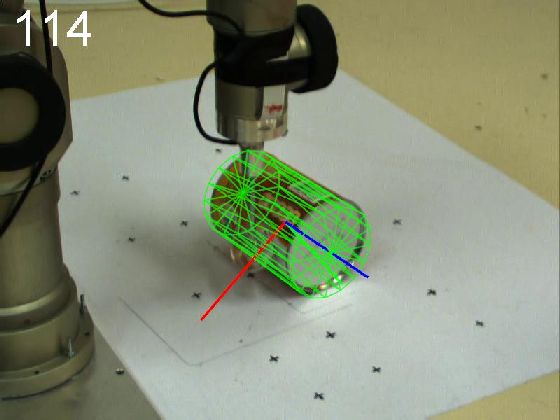
\includegraphics[width=2.3cm]{images/A3_physx_39_2}
% 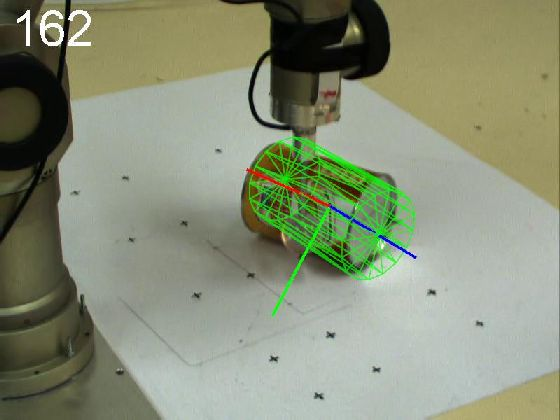
\includegraphics[width=2.3cm]{images/A3_physx_39_3}
% \includegraphics[width=2.3cm]{images/A3_physx_39_4}
% \includegraphics[width=2.3cm]{images/A3_physx_39_5}
% }
% \caption {Experiment L: cylinder.  Green outline shows predictions
%   (from top row to bottom row) by KDEF-GA/quat, LWPR-G, and PhysX for
%   one trial.  A set of axes is attached to the cylinder to show the
%   predicted rotation of the cylinder about its axis.  (The frame
%   number is shown in the top left of each image.)  }
% \label{fig:ExperimentL3}
% \end{figure*}

{\bf Experiment P1 discussion:} We may draw several conclusions. First
from Table~\ref{tab:PerformanceTableL1av} and Figure~\ref{fig:Lgraphs}
it can be seen that the learned models almost always outperformed the
physics simulator on the test set, giving an error approximately one
third the size. Thus we find strong support for hypothesis H1. With respect to parameterisations of density estimation Gaussians with quaternions gave the best performance in 14 of the 15 cases  (Table~\ref{tab:PerformanceTableL1av} boldentries). Thus in experiments P2 and P3 this parameterisation was used
for the density estimation algorithms.
Recall that for LWPR we used an Euler angle parameterisation throughout, as this
provides a lower dimension input space on which the regression method
tends to work best. We verified this in informal experiments not reported here.

% @@@ COMMENT ON KDE-GAX RESULTS
\begin{figure*}[htbp]
\centerline{
\includegraphics[width=\imgAXwid]{images/A1_2exp_667_1}
\includegraphics[width=\imgAXwid]{images/A1_2exp_876_1}
\includegraphics[width=\imgAXwid]{images/A2_2exp_399_1}
\includegraphics[width=\imgAXwid]{images/A2_LWPR1_399_1}
\includegraphics[width=\imgAXwid]{images/A2_2exp_87_1}
\includegraphics[width=\imgAXwid]{images/A3_2exp_39_1}
\includegraphics[width=\imgAXwid]{images/A3_LWPR1_39_1}
\includegraphics[width=\imgAXwid]{images/A3_physx_39_1}
}
%\vspace{0.1cm}
\centerline{
\includegraphics[width=\imgAXwid]{images/A1_2exp_667_2}
\includegraphics[width=\imgAXwid]{images/A1_2exp_876_2}
\includegraphics[width=\imgAXwid]{images/A2_2exp_399_2}
\includegraphics[width=\imgAXwid]{images/A2_LWPR1_399_2}
\includegraphics[width=\imgAXwid]{images/A2_2exp_87_2}
\includegraphics[width=\imgAXwid]{images/A3_2exp_39_2}
\includegraphics[width=\imgAXwid]{images/A3_LWPR1_39_2}
\includegraphics[width=\imgAXwid]{images/A3_physx_39_2}
}
% problem with physx @@@
%\vspace{0.1cm}
%\centerline{
%\includegraphics[width=\imgAXwid]{images/A2_physx_399_1}
%\includegraphics[width=\imgAXwid]{images/A2_physx_399_2}
%\includegraphics[width=\imgAXwid]{images/A2_physx_399_3}
%\includegraphics[width=\imgAXwid]{images/A2_physx_399_4}
%\includegraphics[width=\imgAXwid]{images/A2_physx_399_5}
%}
%\vspace{0.1cm}
\centerline{
\includegraphics[width=\imgAXwid]{images/A1_2exp_667_3}
\includegraphics[width=\imgAXwid]{images/A1_2exp_876_3}
\includegraphics[width=\imgAXwid]{images/A2_2exp_399_3}
\includegraphics[width=\imgAXwid]{images/A2_LWPR1_399_3}
\includegraphics[width=\imgAXwid]{images/A2_2exp_87_3}
\includegraphics[width=\imgAXwid]{images/A3_2exp_39_3}
\includegraphics[width=\imgAXwid]{images/A3_LWPR1_39_3}
\includegraphics[width=\imgAXwid]{images/A3_physx_39_3}
}
\centerline{
\includegraphics[width=\imgAXwid]{images/A1_2exp_667_4}
\includegraphics[width=\imgAXwid]{images/A1_2exp_876_4}
\includegraphics[width=\imgAXwid]{images/A2_2exp_399_4}
\includegraphics[width=\imgAXwid]{images/A2_LWPR1_399_4}
\includegraphics[width=\imgAXwid]{images/A2_2exp_87_4}
\includegraphics[width=\imgAXwid]{images/A3_2exp_39_4}
\includegraphics[width=\imgAXwid]{images/A3_LWPR1_39_4}
\includegraphics[width=\imgAXwid]{images/A3_physx_39_4}
}
%\vspace{0.1cm}
\centerline{
\includegraphics[width=\imgAXwid]{images/A1_2exp_667_5}
\includegraphics[width=\imgAXwid]{images/A1_2exp_876_5}
\includegraphics[width=\imgAXwid]{images/A2_2exp_399_5}
\includegraphics[width=\imgAXwid]{images/A2_LWPR1_399_5}
\includegraphics[width=\imgAXwid]{images/A2_2exp_87_5}
\includegraphics[width=\imgAXwid]{images/A3_2exp_39_5}
\includegraphics[width=\imgAXwid]{images/A3_LWPR1_39_5}
\includegraphics[width=\imgAXwid]{images/A3_physx_39_5}
}
%\vspace{0.1cm}
\caption {Experiment P1: polyflap, box and cylinder. Green outline shows
  predictions. Columns 1-2: KDEF-GA/quat on two trials exhibiting
  different motions of the polyflap. Col 3: KDEF-GA/quat. Col 4: LWPR-G for one trial in
  which the box topples over. Col 5: KDEF-GA/quat on another trial in
  which the box slides. Columns 6-8 show the same push of the
  cylinder. Col 6: KDEF-GA/quat. Col 7: LWPR-G. Col 8: PhysX. Note tha
  for columns 6-7 the orientation of the cylinder is show by the
  rotating frame. Only the learned models predict the rotation
  correctly.(The
  frame number is shown in the top left of each image.)  }
\label{fig:ExperimentL2}
\end{figure*}

In the image sequences
(Figures~\ref{fig:ExperimentL2}) it can be
seen that predictions were accurate and physically plausible for a
variety of learning methods even over 150 steps. Note the physics
simulator predicts incorrect turning of the cylinder when pushed
(Figure~\ref{fig:ExperimentL2} column 8). Finally
Figure~\ref{fig:Lgraphs} also shows the interaction between different
amounts of information in the input space and the learning
algorithm. This shows that when learning about a single object that
regression performance declined slightly as the dimensionality was
increased. It also shows that when learning about a single object
additional information about contacts provides no clear advantage for
any of the learning methods. This is because for a model of a single
object no learning transfer is required. These were the two cases
where it was hypothesized that additional information about contacts
could improve performance. We now turn to these cases in experiments P2
and P3.



%%%%%%%%%%%%%%%%%%%%%%%%%%%%%%%%%%%%%%%%%%%%%%%%%%%%%%%%%%%%%%%%%%%%%%%
%% Experiment A

\subsection{Experiment P2: Action Transfer}
\label{sec:Results.Action}

\begin{figure}[t]
\centerline{\includegraphics[width=0.9\columnwidth]{graphs_jw/A_real_sim_av_graph}}
%\centerline{\includegraphics[width=0.45\columnwidth]{graphs_jw/A_sim_av_graph.png}%}
%\centerline{
%\includegraphics[width=0.46\columnwidth]{graphs_jw/A_real_av_graph.png}}
\centerline{\includegraphics[width=0.9\columnwidth]{graphs_jw/graph_key}}
\caption{Experiment P2: Transfer of learning to novel actions.
Trained on forward push on polyflap, tested on backward push,
for simulated (top) and real data (bottom).
Comparative performance of predictors vs. information utilised
(global/agent/environment),
as measured by the normalised average error ${E_{av}^{norm}}$.
%Also included is a single data point for the PhysX physics engine.
}\label{fig:A_av_graphs}
\end{figure}

%\begin{table}[b]
%\begin{center}
%\begin{tabular}{|l|l|l|l|l|}
%\cline{3-5}
%\multicolumn{2}{c}{ } & \multicolumn{3}{|c|}{Information Utilised} \\
%\cline{1-5}
%Predictor & data & Global\,(G) & G\,\&\,Agent\,(A) & G\,\&\,A\,\&\,Env \\
%\cline{1-5}
%KDEF & sim & 0.155$\pm$0.001 & 0.036$\pm$0.002 & \textbf{0.023}$\pm$0.001 \\
%LWPR & sim & 0.139$\pm$0.001 & 0.139$\pm$0.001 & 0.139$\pm$0.001 \\
%KDE & sim & n/a & 0.152$\pm$0.001& 0.147$\pm$0.001 \\
%\cline{1-5}
%KDEF & real & 0.133$\pm$0.002 & \textbf{0.097}$\pm$0.004 & 0.132$\pm$0.008 \\
%LWPR & real & 0.130$\pm$0.002 & 0.130$\pm$0.002 & 0.130$\pm$0.002 \\
%KDE & real & n/a & 0.133$\pm$0.002 & 0.140$\pm$0.002 \\
%\cline{3-5}
%PhysX & real & \multicolumn{3}{|c|}{0.143$\pm$0.008} \\
%\cline{1-5}
%\end{tabular}
%\end{center}
%\caption[Performance Table]{Experiment A: Generalisation to novel action.
%Trained on forward push on polyflap, tested on backward push, for simulated and real data.
%Comparative performance of predictors vs. information used.
%Shown is the dimensionless measure normalised average error ${E_{av}^{norm}} \pm$ standard error.
%}\label{tab:PerformanceTableAav}
%\end{table}

Experiment P2 tests hypothesis H2: whether predictions can be
transfered to novel actions, i.e.\ to those that fall outside the
convex hull of actions in the training set.  The predictors were
trained with 900 examples of pushes applied to a polyflap in one
direction relative to the polyflap (Figure~\ref{fig:ToyExample} top
left).  Predictors were then tested on 100 examples of pushes applied
in the opposite direction (Figure~\ref{fig:ToyExample} top
right). Gaussian kernels with quaternion parameterisation were used
for the density estimation methods, and an Euler angle representation
with LWPR. The same method was followed in simulation and with the
real object. In the real case we tested all the algorithm-information
variants in Table~\ref{tab:algs}. In simulation we tested all the
variants except the PhysX simulator, which provided the simulation
environment. In each case the error measured is the transfer
prediction error, i.e.\ the prediction error for the novel test
actions.
%In each case, we test performance according to the information utilised:
%global only, global and agent, or global, agent and environment,
%which for KDEF correspond to the -G, -GA and -GAE cases respectively.
%Also shown are the results from KDE\mbox{-}GA and KDE\mbox{-}GAE.

Figure~\ref{fig:A_av_graphs} %(also see Table~\ref{tab:PerformanceTableAav})
shows the normalised average error $E_{av}^{norm}$ for tests carried
out in simulation (left panel) and with real objects (right panel).
Figure~\ref{fig:ExperimentA} shows example predicted trajectories on
synthetic and real test cases.

% @@@ COMMENT ON KDE-GAX RESULTS
% \begin{figure*}[tbp]
% \centerline{
% \includegraphics[width=2.3cm]{images/B1_1exp_20_1}
% \includegraphics[width=2.3cm]{images/B1_1exp_20_2}
% \includegraphics[width=2.3cm]{images/B1_1exp_20_3}
% \includegraphics[width=2.3cm]{images/B1_1exp_20_4}
% \includegraphics[width=2.3cm]{images/B1_1exp_20_5}
% }
% \vspace{0.1cm}
% \centerline{
% \includegraphics[width=2.3cm]{images/B1_2exp_20_1}
% \includegraphics[width=2.3cm]{images/B1_2exp_20_2}
% \includegraphics[width=2.3cm]{images/B1_2exp_20_3}
% \includegraphics[width=2.3cm]{images/B1_2exp_20_4}
% \includegraphics[width=2.3cm]{images/B1_2exp_20_5}
% }
% \vspace{0.1cm}
% \centerline{
% \includegraphics[width=2.3cm]{images/B1_3exp_20_1}
% \includegraphics[width=2.3cm]{images/B1_3exp_20_2}
% \includegraphics[width=2.3cm]{images/B1_3exp_20_3}
% \includegraphics[width=2.3cm]{images/B1_3exp_20_4}
% \includegraphics[width=2.3cm]{images/B1_3exp_20_5}
% }
% %\vspace{0.1cm}
% %\centerline{
% %\includegraphics[width=2.3cm]{images/B1_3exp_61_1}
% %\includegraphics[width=2.3cm]{images/B1_3exp_61_2}
% %\includegraphics[width=2.3cm]{images/B1_3exp_61_3}
% %\includegraphics[width=2.3cm]{images/B1_3exp_61_4}
% %\includegraphics[width=2.3cm]{images/B1_3exp_61_5}
% %}
% \caption
% {Experiment A (simulation):
% Green outline shows predictions (from top row to bottom row) by

% compared to simulated `ground truth' (in cyan).
% These predictions illustrate the rationale for extra contact information
% presented in Figure~\ref{fig:ToyExample}.
% (The frame number is shown in the top left of each image.)
% }
% \label{fig:ExperimentA}
% \end{figure*}

\newlength{\imgBXwid}
\setlength{\imgBXwid}{2.15cm}
\begin{figure*}[tb]
\centerline{
\includegraphics[width=\imgBXwid]{images/B1_1exp_20_1}
\includegraphics[width=\imgBXwid]{images/B1_2exp_20_1}
\includegraphics[width=\imgBXwid]{images/B1_3exp_20_1}
\includegraphics[width=\imgBXwid]{images/B2_2exp_58_1}
\includegraphics[width=\imgBXwid]{images/B2_1exp_58_1}
\includegraphics[width=\imgBXwid]{images/B2_LWPR1_58_1}
\includegraphics[width=\imgBXwid]{images/B2_2exp_38_1}
}
%\vspace{0.1cm}
\centerline{
\includegraphics[width=\imgBXwid]{images/B1_1exp_20_2}
\includegraphics[width=\imgBXwid]{images/B1_2exp_20_2}
\includegraphics[width=\imgBXwid]{images/B1_3exp_20_2}
\includegraphics[width=\imgBXwid]{images/B2_2exp_58_2}
\includegraphics[width=\imgBXwid]{images/B2_1exp_58_2}
\includegraphics[width=\imgBXwid]{images/B2_LWPR1_58_2}
\includegraphics[width=\imgBXwid]{images/B2_2exp_38_2}
}
%\vspace{0.1cm}
\centerline{
\includegraphics[width=\imgBXwid]{images/B1_1exp_20_3}
\includegraphics[width=\imgBXwid]{images/B1_2exp_20_3}
\includegraphics[width=\imgBXwid]{images/B1_3exp_20_3}
\includegraphics[width=\imgBXwid]{images/B2_2exp_58_3}
\includegraphics[width=\imgBXwid]{images/B2_1exp_58_3}
\includegraphics[width=\imgBXwid]{images/B2_LWPR1_58_3}
\includegraphics[width=\imgBXwid]{images/B2_2exp_38_3}
}

\centerline{
\includegraphics[width=\imgBXwid]{images/B1_1exp_20_4}
\includegraphics[width=\imgBXwid]{images/B1_2exp_20_4}
\includegraphics[width=\imgBXwid]{images/B1_3exp_20_4}
\includegraphics[width=\imgBXwid]{images/B2_2exp_58_4}
\includegraphics[width=\imgBXwid]{images/B2_1exp_58_4}
\includegraphics[width=\imgBXwid]{images/B2_LWPR1_58_4}
\includegraphics[width=\imgBXwid]{images/B2_2exp_38_4}
}
%\vspace{0.1cm}
\centerline{
\includegraphics[width=\imgBXwid]{images/B1_1exp_20_5}
\includegraphics[width=\imgBXwid]{images/B1_2exp_20_5}
\includegraphics[width=\imgBXwid]{images/B1_3exp_20_5}
\includegraphics[width=\imgBXwid]{images/B2_2exp_58_5}
\includegraphics[width=\imgBXwid]{images/B2_1exp_58_5}
\includegraphics[width=\imgBXwid]{images/B2_LWPR1_58_5}
\includegraphics[width=\imgBXwid]{images/B2_2exp_38_5}
}
\caption
{Experiment P2: Green outline shows predictions. Column 1: KDEF-G/quat. Col 2:
KDEF-GA/quat. Col 3: KDEF-GAE/quat. Col 4: KDEF-GA/quat. Col 5:
KDEF-G/quat. Col 6: LWPR-G. Col 7: KDEF-GA/quat.
Note that the KDEF-G/quat and LWPR-G methods predict
that the robot finger passes through the polyflap.
(The frame number is shown in the top left of each image.)
}
\label{fig:ExperimentA}
\end{figure*}

{\bf Experiment P2 discussion:} The following conclusions may be
drawn. Figure~\ref{fig:A_av_graphs} (left panel) shows that in
simulation the unfactored KDE and LWPR algorithms had roughly constant
transfer prediction error irrespective of increasing information. In contrast
the transfer error of KDEF reduced significantly as information about
finger-object and object-environment relations was added. The
predictions (Figure~\ref{fig:ExperimentA}) matched the hypothesised
behaviour from Figure~\ref{fig:ToyExample} (bottom row). With only
global information the finger was predicted to pass through the object
(Figure~\ref{fig:ExperimentA} column 1). By adding the agent-object
information and modelling its effect as a separate factor, the
prediction was that the object would move with the finger, but that it
penetrated the table (Figure~\ref{fig:ExperimentA} column 2). By also
adding object-environment information the prediction prevented this
penetration so that the object will move along the table with the
finger (Figure~\ref{fig:ExperimentA} column 3).

On real data (Figure~\ref{fig:A_av_graphs} right panel) the transfer
performance of the learned predictors was slightly better than the
prediction error of the physics engine. All the methods had roughly
constant performance except for the factored version. Its advantage
no longer held when information G+A+E was used, but it retained some
advantage with information G+A. Figure~\ref{fig:ExperimentA}
(columns 5 and 6) shows that learners (KDEF, LWPR) with information G
predict, as in simulation, that the finger passes through the object,
and that the object doesn't move at all. In
Figure~\ref{fig:ExperimentA} (columns 4 and 7) the KDEF predictor
with information G+A correctly predicts the sliding motion of the
object, although it fails to capture the slight rotation. Collectively
these results provide support for hypothesis H2q, but information GAE is required for best performance provided the observations are reliable. In addition only
the factored KDE formulation was able to exploit this additional
information, either in simulation or for real objects. 
%data, it is clear that LWPR fails to generalise in this way -- it
%predicts that the polyflap will never move at all, because it was
%never exposed to these kinds of pushes during training.  The
%single-factor KDE variant exhibits a similar level of normalised
%average error.
%In contrast, the KDEF method is able to make physically plausible predictions,
%which are accurate enough to be useful for planning manipulative pushes.
%We note that, with simulated data, the -GAE method does better than
%the -GA method, whereas, with real data, the converse is true.  We
%suggest that this discrepancy is again due to inaccuracies in the
%visual tracking system.


%%%%%%%%%%%%%%%%%%%%%%%%%%%%%%%%%%%%%%%%%%%%%%%%%%%%%%%%%%%%%%%%%%%%%%%
%% Experiment S1

\subsection{Experiment P3:  Shape Transfer}\label{sec:Results.Shape}

Experiment P3
%consists of two experiments S-interpolation and
%S-transfer. The first tests hypothesis H3 a), by measuring
%generalisation error when a range of shapes are presented in training,
%and the test shapes fall within that variation, requiring
%interpolative generalisation. The second 
tests hypothesis H3, by
measuring whether predictors learned from one or two objects can
transfer their predictions to an object of novel shape.

%\subsubsection{S-interpolation}
%
%%\todo[color=\JW,inline]{rewrite or update this section on S3}
%
%This experiment was performed only in simulation. All training and
%test data involved polyflaps constructed from two square plates.  A
%set of polyflaps was generated by randomising the angle at which the
%plates connect.  Even a small angular variation can alter the
%behaviour of the object significantly. As
%Figure~\ref{fig:ExperimentS3Setup} shows, a downwards push from above
%will cause the entire object to move either left or right,
%depending on small changes in the angle of the plates. The training
%was carried out on 900 downward pushes of polyflaps with angles
%varying uniformly around $90^\circ$ by $\pm 70^\circ$, and tested on
%100 new polyflaps drawn from the same distribution.
%Figure~\ref{fig:S_av_graphs} (bottom right) shows the normalised
%average error $E_{av}^{norm}$ for methods KDEF, LWPR and KDE-GA, as
%the information available varies, with further detail in
%Table~\ref{tab:PerformanceTableS3av}. Specific predictions are shown in
%Figure~\ref{fig:ExperimentS3}.
%
%{\bf S-interpolation discussion:} The experiment reveals that adding
%additional information (GA or GAE) significantly reduces
%generalisation error. Figure~\ref{fig:ExperimentS3} (column 1) shows
%that only using global information G gives inadequate predictions
%because shape changes are not accounted for, whereas columns 2 and 3
%show qualitatively correct predictions when they are. All three
%learning frameworks are able to exploit this information.
%
%\begin{figure}[t]
%\centerline{
%\includegraphics[width=2.3cm]{E6_backReg}
%\includegraphics[width=2.3cm]{E6_back}
%\includegraphics[width=2.3cm]{E6_front}
%}
%\caption[Experiment S-interpolative] {Experiment
%  S-interpolative. These images show training data for this experiment
%  in which a fingertip (grey ball) descended onto a polyflap from
%  above. Small variations in the fold angle of the polyflap can lead
%  to quite different object motions, given identical pushes from the
%  fingertip. When the polyflap is folded acutely, the fingertip will
%  push it to the left, whereas with a fold angle greater than ninety
%  degrees, the same push will move the polyflap to the right.}
%\label{fig:ExperimentS3Setup}
%\end{figure}
%
%\subsubsection{S-transfer}
%
%In Experiment~S-transfer, w
The experiment was run in simulation and with real objects. We
perform the same experiment testing learning transfer from i) a
polyflap to a box and ii) a box and a cylinder to a double
cylinder. There were 900 training pushes on the polyflap and 200 test
pushes on the box for i), and 200 training pushes (100 box, 100
cylinder) and 100 test pushes (double cylinder) for ii). This experiment ran on real
objects for i) and ii) and in simulation only for i), giving three
train-test conditions in total. We have previously published results
from simulation for i) \cite{kopicki-etal-icra11}. A
Gaussian-quaternion parameterisation was used for the density
estimation methods and an Euler angle parameterisation for LWPR. All
algorithm-information combinations from Table~\ref{tab:algs} were
tried. When learning from two objects the same number of factors
(experts) were used for each object, and they were matched across the
two objects by hand. This means each expert received a mix of data
from each object, learning to encode both rolling and sliding or
tipping motions. %In Experiment S2, we make use of a ``double cylinder'' object,
%which consists of two cylinders which have been rigidly joined together
%This poses a considerable challenge for many learned predictors.
%For example, a predictor that uses only global information
%when trained on a single cylinder will predict that cylinders tend to rotate --
%such a predictor may predict that the double cylinder object should also rotate,
%when in practice it is constrained to slide without rolling.
The normalised average error for all three conditions $E_{av}^{norm}$
is shown in Figure~\ref{fig:S_av_graphs}. %and in
%Tables~\ref{tab:PerformanceTableS1av}-\ref{tab:PerformanceTableS2av}. 
Example frames from the experiments are shown in
Figure~\ref{fig:ExperimentStransfer}.

%\begin{table}[b]
%\begin{center}
%\begin{tabular}{|l|l|l|l|}
%\cline{2-4}
%\multicolumn{1}{c}{ } & \multicolumn{3}{|c|}{Information Utilised} \\
%\cline{1-4}
%Predictor & Global\,(G) & G\,\&\,Agent\,(A) & G\,\&\,A\,\&\,Env \\
%\cline{1-4}
%KDEF & 0.060$\pm$0.002 & 0.018$\pm$0.002 & 0.026$\pm$0.003 \\
%LWPR & 0.063$\pm$0.001 & 0.061$\pm$0.001 & 0.025$\pm$0.001 \\
%KDE & n/a & \textbf{0.017}$\pm$0.001 & 0.018$\pm$0.001 \\
%\cline{1-4}
%\end{tabular}
%\end{center}
%\caption[Performance Table]{Experiment S-interpolative: generalisation to novel shape.
%Trained with down pushes on angled polyflaps, tested on similar polyflaps, using simulated data.
%Comparative performance of predictors vs. information used.
%Shown is the dimensionless measure normalised average error ${E_{av}^{norm}}$.
%}\label{tab:PerformanceTableS3av}
%\end{table}

%\newlength{\imgDXwid}
%\setlength{\imgDXwid}{2.15cm}
%
%\begin{figure}[t]
%\centerline{
%\includegraphics[width=\imgDXwid]{images/D1_1exp_594_1}
%\includegraphics[width=\imgDXwid]{images/D1_2exp_594_1}
%\includegraphics[width=\imgDXwid]{images/D1_LWPR2_594_1}
%}
%%\vspace{0.1cm}
%\centerline{
%\includegraphics[width=\imgDXwid]{images/D1_1exp_594_2}
%\includegraphics[width=\imgDXwid]{images/D1_2exp_594_2}
%\includegraphics[width=\imgDXwid]{images/D1_LWPR2_594_2}
%}
%%\vspace{0.1cm}
%\centerline{
%\includegraphics[width=\imgDXwid]{images/D1_1exp_594_3}
%\includegraphics[width=\imgDXwid]{images/D1_2exp_594_3}
%\includegraphics[width=\imgDXwid]{images/D1_LWPR2_594_3}
%}
%\centerline{
%\includegraphics[width=\imgDXwid]{images/D1_1exp_594_4}
%\includegraphics[width=\imgDXwid]{images/D1_2exp_594_4}
%\includegraphics[width=\imgDXwid]{images/D1_LWPR2_594_4}
%}
%\centerline{
%\includegraphics[width=\imgDXwid]{images/D1_1exp_594_5}
%\includegraphics[width=\imgDXwid]{images/D1_2exp_594_5}
%\includegraphics[width=\imgDXwid]{images/D1_LWPR2_594_5}
%}
%\caption {Experiment S-interpolation (simulation) reveals limitations
%  of the methods using only global information, which fail to predict
%  the motion of an angled polyflap when subjected to a downward push.
%  The augmented input methods can cope well with this kind of shape
%  variation.  Green outline shows predictions (left to right column)
%  by KDEF-G/quat, KDEF-GA/quat, and LWPR-GA, compared to simulated
%  `ground truth' (in cyan).  (The frame number is shown in the top
%  left of each image.)  }
%\label{fig:ExperimentS3}
%\end{figure}

{\bf Experiment P3 discussion:} 
%We see that KDEF performs best, according
%to the normalised average error measure.  As with Experiment~A, for
%the simulated data (assuming perfect visual tracking) the KDEF-GAE
%performs best, suggesting that this technique will dominate with a
%high-precision vision system.  For the tests with real data, all
%techniques suffer from poor accuracy.  However, the KDEF methods
%(KDEF\mbox{-}GA and KDEF\mbox{-}GAE) give physically plausible
%predictions, while the LWPR technique predicts that the box will
%remain stationary throughout the pushing sequence.
The easier transfer case is from polyflap to box, here the range of
motions for the polyflap from one direction are similar to those for a
box. Even so the actual transferred learner predictions are physically
plausible only when additional information is present, such as for the
KDEF-GA method (Figure~\ref{fig:ExperimentStransfer} column 1). In
this experiment KDEF-G and LWPR-G again wrongly predict finger motion
through the box in columns 2 and 3. The harder transfer case is to
learn from two different objects (box and cylinder) and transfer to
one quite different object (double cylinder). In this case only the
KDEF-GAE method was able to produce physically plausible
predictions. In Figure~\ref{fig:ExperimentStransfer} (column 6) the
prediction is of the double-cylinder sliding along the table, whereas
KDEF with information G or G+A makes physically implausible
predictions of interpenetration with the table
(Figure~\ref{fig:ExperimentStransfer} columns 4 and 5). That the
predictions are plausible with real data is shown in
Figure~\ref{fig:ExperimentStransfer}. These results collectively
provide support that only using information G+A+E is sufficient to
achieve learning transfer to novel shapes, with that entailing both
low prediction errors and physically plausible predictions. In
addition only the factored formulation of KDE was able to take
advantage of this information. Thus this experiment provides support
for hypothesis H3 for the case of KDEF-GAE only.

%***ADD IMAGES TO ILLUSTRATE HOW LWPR ALWAYS REMAINS STATIONARY WHILE KDE PREDICTS MOTIONS!!!***

% @@@ COMMENT ON KDE-GAX RESULTS



%%%%%%%%%%%%%%%%%%%%%%%%%%%%%%%%%%%%%%%%%%%%%%%%%%%%%%%%%%%%%%%%%%%%%%%
%% Experiment S2

%\subsubsection{Training on a box and a cylinder, and testing on two rigidly connected cylinders}


% @@@ COMMENT ON KDE-GAX RESULTS

% PROBLEM THAT C5 TRAINED ON ONLY 100 box + 100 cyl
% whereas C2 trained on 500 box + 100 cyl


%\begin{figure}[htbp]
%\centerline{\includegraphics[width=\the\barchartwidth]{S2_sim_av_graph}}
%\centerline{\includegraphics[width=\the\barchartwidth]{S2_real_av_graph}}
%\caption{Experiment S2: Generalisation to novel shape.
%Trained on cylinder and box, tested on double-cylinder,
%for simulated (top) and real data (bottom).%
%Comparative performance of predictors vs. information utilised,
%as measured by the normalised average error ${E_{av}^{norm}}$.}
%\label{fig:S2_av_graphs}
%\end{figure}


% @@@ COMMENT ON KDE-GAX RESULTS, WHICH ARE THE BEST !!!

%\begin{figure}[htbp]
%\centerline{\includegraphics[width=\the\barchartwidth]{graphs_jw/S3_sim_av_graph.png}}
%\caption{Experiment S3: Interpolative generalisation to novel shape.
%Trained with downward pushes on angled polyflaps,
%tested on similar polyflaps, using simulated data.
%Comparative performance of predictors vs. information utilised,
%as measured by the normalised average error ${E_{av}^{norm}}$.}
%\label{fig:S3_av_graph}
%\end{figure}


% \begin{figure*}[htbp]
% \centerline{
% \includegraphics[width=2.3cm]{images/C5_1exp_6_1}
% \includegraphics[width=2.3cm]{images/C5_1exp_6_2}
% \includegraphics[width=2.3cm]{images/C5_1exp_6_3}
% \includegraphics[width=2.3cm]{images/C5_1exp_6_4}
% \includegraphics[width=2.3cm]{images/C5_1exp_6_5}
% }
% \vspace{0.1cm}
% \centerline{
% \includegraphics[width=2.3cm]{images/C5_2exp_6_1}
% \includegraphics[width=2.3cm]{images/C5_2exp_6_2}
% \includegraphics[width=2.3cm]{images/C5_2exp_6_3}
% \includegraphics[width=2.3cm]{images/C5_2exp_6_4}
% \includegraphics[width=2.3cm]{images/C5_2exp_6_5}
% }
% \vspace{0.1cm}
% \centerline{
% \includegraphics[width=2.3cm]{images/C5_3exp_6_1}
% \includegraphics[width=2.3cm]{images/C5_3exp_6_2}
% \includegraphics[width=2.3cm]{images/C5_3exp_6_3}
% \includegraphics[width=2.3cm]{images/C5_3exp_6_4}
% \includegraphics[width=2.3cm]{images/C5_3exp_6_5}
% }
% %\vspace{0.1cm}
% %\centerline{
% %\includegraphics[width=2.3cm]{images/C5_3exp_12_1}
% %\includegraphics[width=2.3cm]{images/C5_3exp_12_2}
% %\includegraphics[width=2.3cm]{images/C5_3exp_12_3}
% %\includegraphics[width=2.3cm]{images/C5_3exp_12_4}
% %\includegraphics[width=2.3cm]{images/C5_3exp_12_5}
% %}
% \caption {Experiment S-transfer: extrapolative generalisation to novel
%   shape (simulation): Green outline shows predictions (from top row to
%   bottom row) by KDEF-G/quat, KDEF-GA/quat, and KDEF-GAE/quat,
%   compared to simulated `ground truth' (in cyan).  Note that the -G
%   and -GA methods predict that the object moves into and through the
%   ground plane.  (The frame number is shown in the top left of each
%   image.)  }
% %\todo[color=\MK,inline]{MK: generate side pushes for S2sim (=C5)}
% \label{fig:ExperimentStransfer}
% \end{figure*}


% \begin{figure*}[htbp]
% %\centerline{
% %\includegraphics[width=2.3cm]{images/C2_3exp_27_1}
% %\includegraphics[width=2.3cm]{images/C2_3exp_27_2}
% %\includegraphics[width=2.3cm]{images/C2_3exp_27_3}
% %\includegraphics[width=2.3cm]{images/C2_3exp_27_4}
% %\includegraphics[width=2.3cm]{images/C2_3exp_27_5}
% %}
% %\vspace{0.1cm}
% \centerline{
% \includegraphics[width=2.3cm]{images/C2_3exp_75_1}
% \includegraphics[width=2.3cm]{images/C2_3exp_75_2}
% \includegraphics[width=2.3cm]{images/C2_3exp_75_3}
% \includegraphics[width=2.3cm]{images/C2_3exp_75_4}
% \includegraphics[width=2.3cm]{images/C2_3exp_75_5}
% }
% \caption {Experiment S-transfer: extrapolative generalisation to novel
%   shape (real data): Green outline shows prediction by KDEF-GAE/quat.
%   (The frame number is shown in the top left of each image.)  }
% \label{fig:ExperimentStransfer}
% \end{figure*}







%\clearpage

%%%%%%%%%%%%%%%%%%%%%%%%%%%%%%%%%%%%%%%%%%%%%%%%%%%%%%%%%%%%%%%%%%%%%%%
%
%${E_{av}^{norm}} \pm se$
%C4.polyflap.1explf & 0.097 $\pm$ 0.002 \\

%${E_{f}^{norm}} \pm se$
%C4.polyflap.1explf & 0.257 $\pm$ 0.006 \\

